\chapter{Results, Discussion and Future Scope}
\label{ch:Results-Discussion-and-Future-Scope}

\section{Experimental Setup}
The mobile robot platform used in this study is custom-tailored by fellow students at Aerospace System Laboratory at the University of Texas at Arlington. It is made from aluminum chassis with fours wheel driven by four gear motors at each wheel. It is equipped with an aluminum shock-absorbing suspension to be used in rough terrain. The rover is equipped with an Intel real sense L-515 LiDAR camera and a stereo camera with two Sony IMX 179 image sensors. Intel NUC is used for on-board processing. The mounting of these optical sensors and Intel NUC are 3D printed from Acrylonitrile Butadiene Styrene (ABS) material. The complete setup is illustrated in Fig.\ref{setup}.  

\section{YOLO-v3 Supervised Training}

\begin{figure}
    \centering
    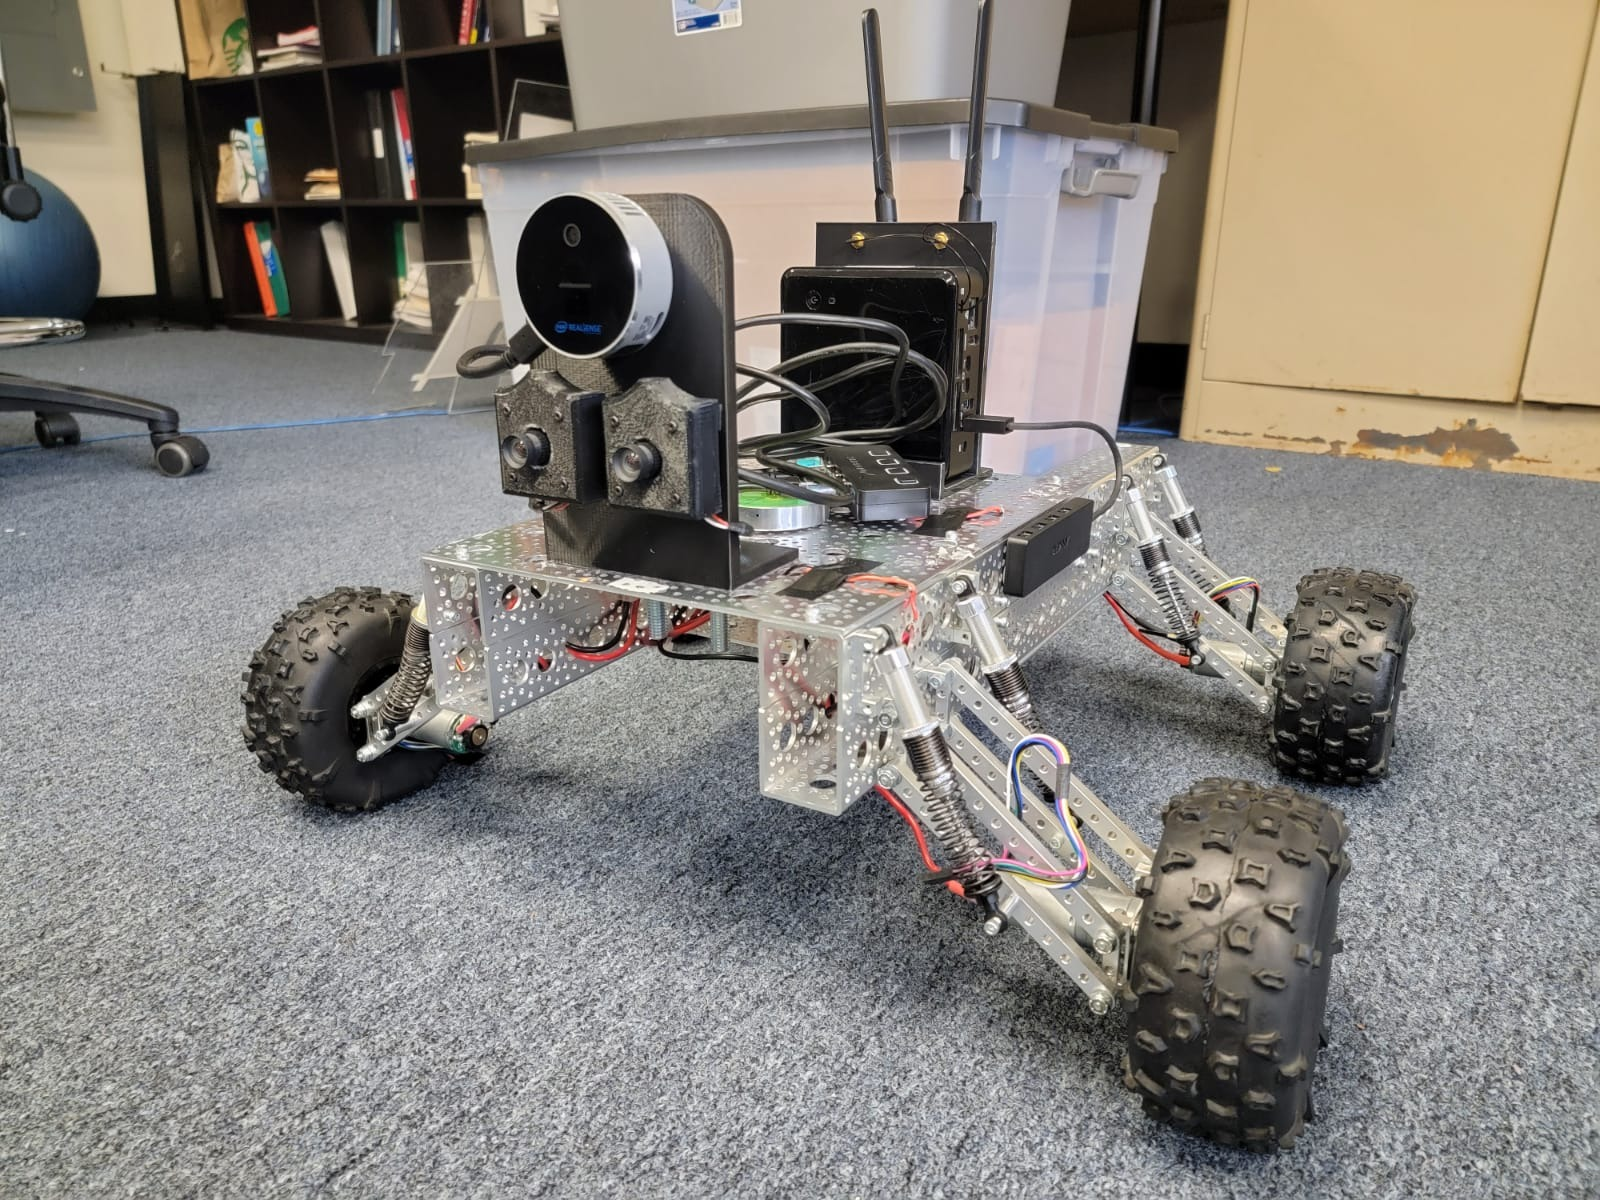
\includegraphics[width=0.8\textwidth]{Images/setup.png}
    \caption{Wheeled Mobile Robot equipped with LiDAR and Stereo Camera}
    \label{setup}
\end{figure}

\begin{figure}
    \centering
    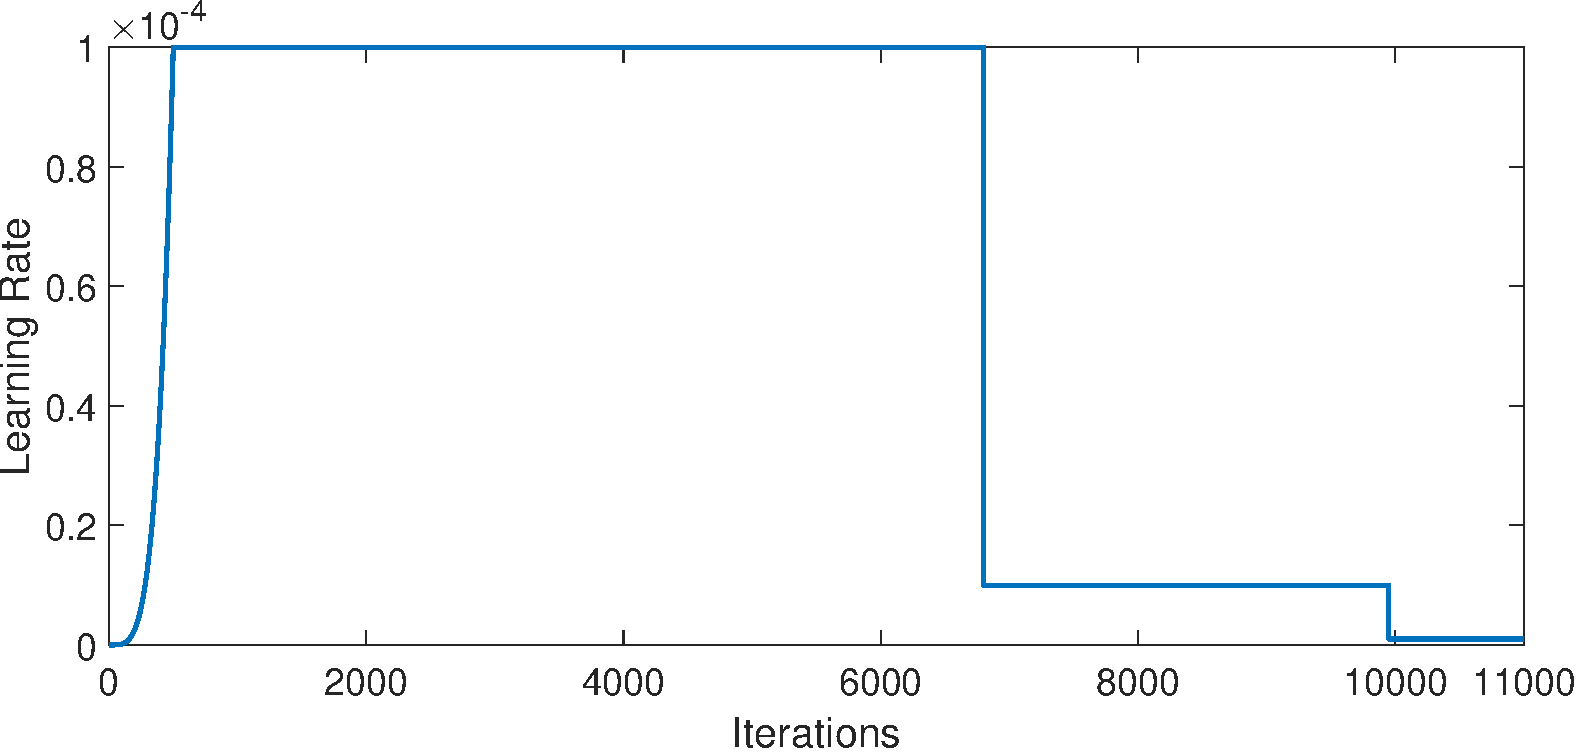
\includegraphics[width=0.9\textwidth]{Images/LearningRate.pdf}
    \caption{Learning Rate Variation During Training}
    \label{learningrate}
\end{figure}

\begin{figure}
    \centering
    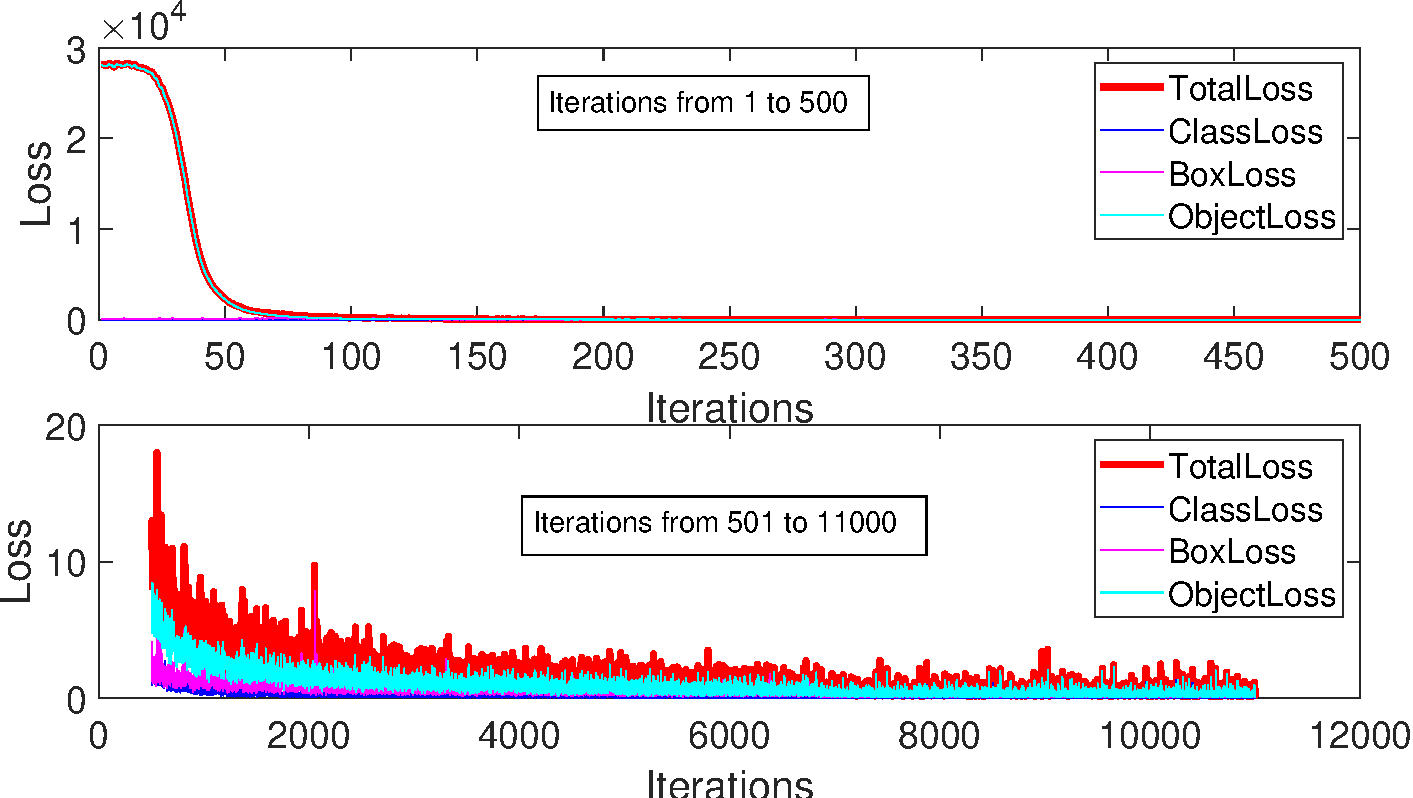
\includegraphics[width=0.9\textwidth]{Images/Loss.pdf}
    \caption{Loss Reduction During Training}
    \label{loss}
\end{figure}

The YOLO-v3 network was trained on custom training data-set with total number of 10989 images. The training data is created to classify and detect four different classes of objects as follows cylinder, Traffic cone, pyramid, and box. Supervised training is performed on the structured dataset which was organise in the form of $y = f(x)$ in order to find the prediction function $\hat{y} = f(x)$ with minimal error $e = min(\hat{y} - y)$. The optimal values of the hyperparameter set for this training are given in table \ref{opthyper}. 

The ground truth dataset is divided into two batches, training and testing batch. From the empirical results, it has been suggested to use few hundreds of image data for the test batch. Since the size of available ground truth data is a total of 10989, the size of the test batch is selected to be 2\% of total data available and the rest of the data is allocated to the training batch.  

Before the start of the training, the bounding boxes from the ground truth data are used as a reference to estimate the anchor boxes, using the k-means clustering algorithm, that precisely fit the training data. The mean IoU of the estimated anchor boxes is 0.8738, this is because of the 12 anchor boxes per detection head (Refer Section 4.5). 

The training is performed in two parts. Initially, the learning rate is low in and is exponentially increased to the preset optimal learning rate till the number of iterations allocated for warming up phase as shown in Fig. \ref{learningrate}. The warm-up period is set to prevent the primacy effect in training. In the initial phase of learning, the SGDM algorithm calculates the gradient based on the initial batches of data which is not accurate and may diverge from the direction to global optima. It can be observed from Fig. \ref{loss} that the loss function value is $30000$ initially, and decreases to 5.46 in this period.

In the second part of training, the learning rate decay is predefined in which the learning rate reduces in discretized steps after a certain number of iterations as seen in Fig.\ref{learningrate}. When near to the end of learning or when the gradient is close to the global optimum, it is suggested from the empirical studies to take small steps toward the global minimum to prevent the gradient to swing around the global minimum. In this part, the network parameters are tuned so that the network can  precisely classify and detect the objects. 

As seen in Fig.\ref{loss}, the training is highly noisy because of the small mini-batch size. However, for the higher value of mini-batch, the training cannot be performed due to insufficient graphics memory of the system. Therefore, the optimum value of mini-batch size is 10 based on the availability of the computational resources. On the other hand, the training on CPU provides flexibility to select a mini-batch size of our choice, although it is expensive in terms of computational time. In this case, training on CPU may take 5-7 days approximately while on GPU it takes 7-8 hours.

\begin{table}
    \centering
    \begin{tabular}{|c|c|c|}
        \hline
        \textbf{Hyperparameter Name} & \textbf{Optimal Value} \\
        \hline
        Numbers of Iterations & 11000 \\
        \hline
        Learning Rate & 0.0001 \\
        \hline
        Warm-up Period & 500 iterations \\
        \hline
        L2 Regularization Parameter & 0.0005 \\
        \hline  
        Mini-batch Size & 10 \\
        \hline
        Train batch & 98\% \\
        \hline
        Test batch & 2\% \\
        \hline 
        Mean IoU of Anchor Box Estimation & 0.8738 \\
        \hline
    \end{tabular}
    \caption{Optimal Value of Hyperparameter Set Considered in Training}
    \label{opthyper}
\end{table}

\section{Neural Network Testing}
Testing of the neural network is performed on the data which is never seen by the network during training. Therefore, 2\% of the ground truth data was kept away for the network performance evaluation. In testing, the trained YOLO-v3 network correctly detects the objects from 201 test images out of 220 images. The pie-chart in Fig.\ref{piechart}(a) illustrates the distribution of test data into correct and faulty detections; additionally, the pie-chart in Fig.\ref{piechart}(b) shows the distribution of sources of error for faulty detections. The major reason for defective detection is multiple detections for single objects. Few other reasons for defective detections could be the network not detecting the object and motion blur. The correct detection results are shown in Fig.\ref{testdetection} with their performance parameters in table \ref{tdp}, and faulty detection examples are shown in Fig.\ref{faultydetection}.   

\begin{figure}
    \centering
    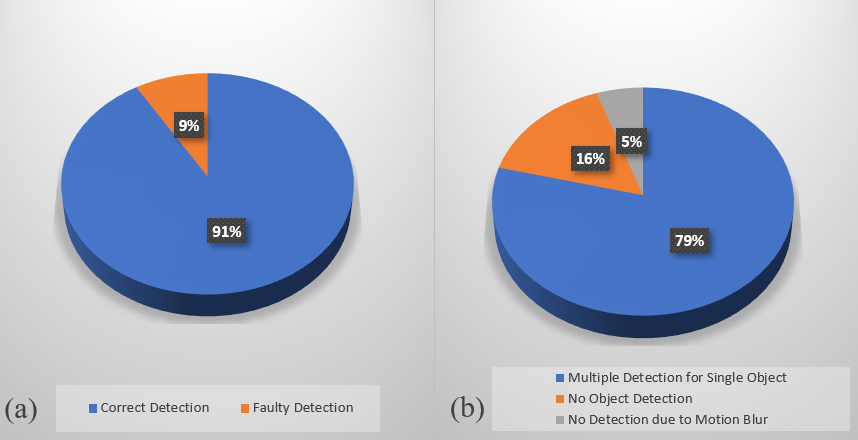
\includegraphics[width=0.9\textwidth]{Images/piechart.png}
    \caption{Pie Chart of Test Results (a) \% of Faulty Detection and (b) \% of Faulty Detection due to Various Reasons}
    \label{piechart}
\end{figure}

\begin{figure}
    \centering
    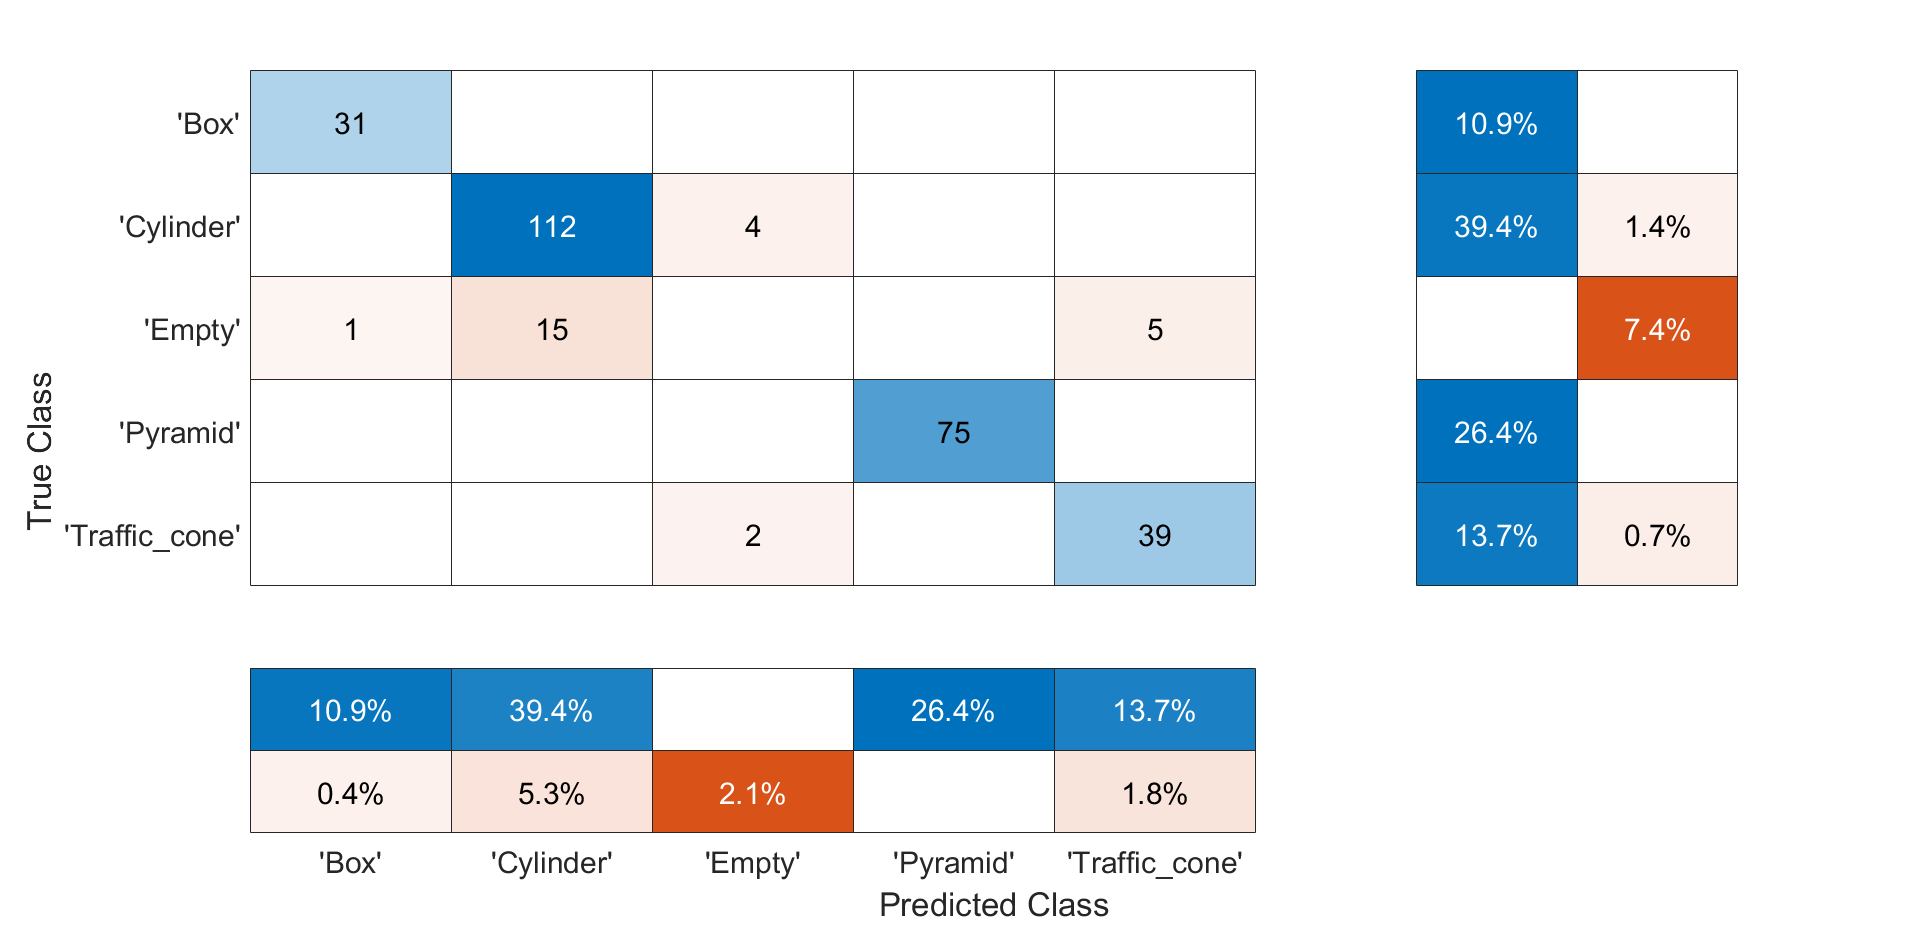
\includegraphics[width=0.9\textwidth]{Images/confusionchart.png}
    \caption{Confusion Chart of Classification on Test Batch}
    \label{confusionchart}
\end{figure}

\begin{figure}
    \centering
    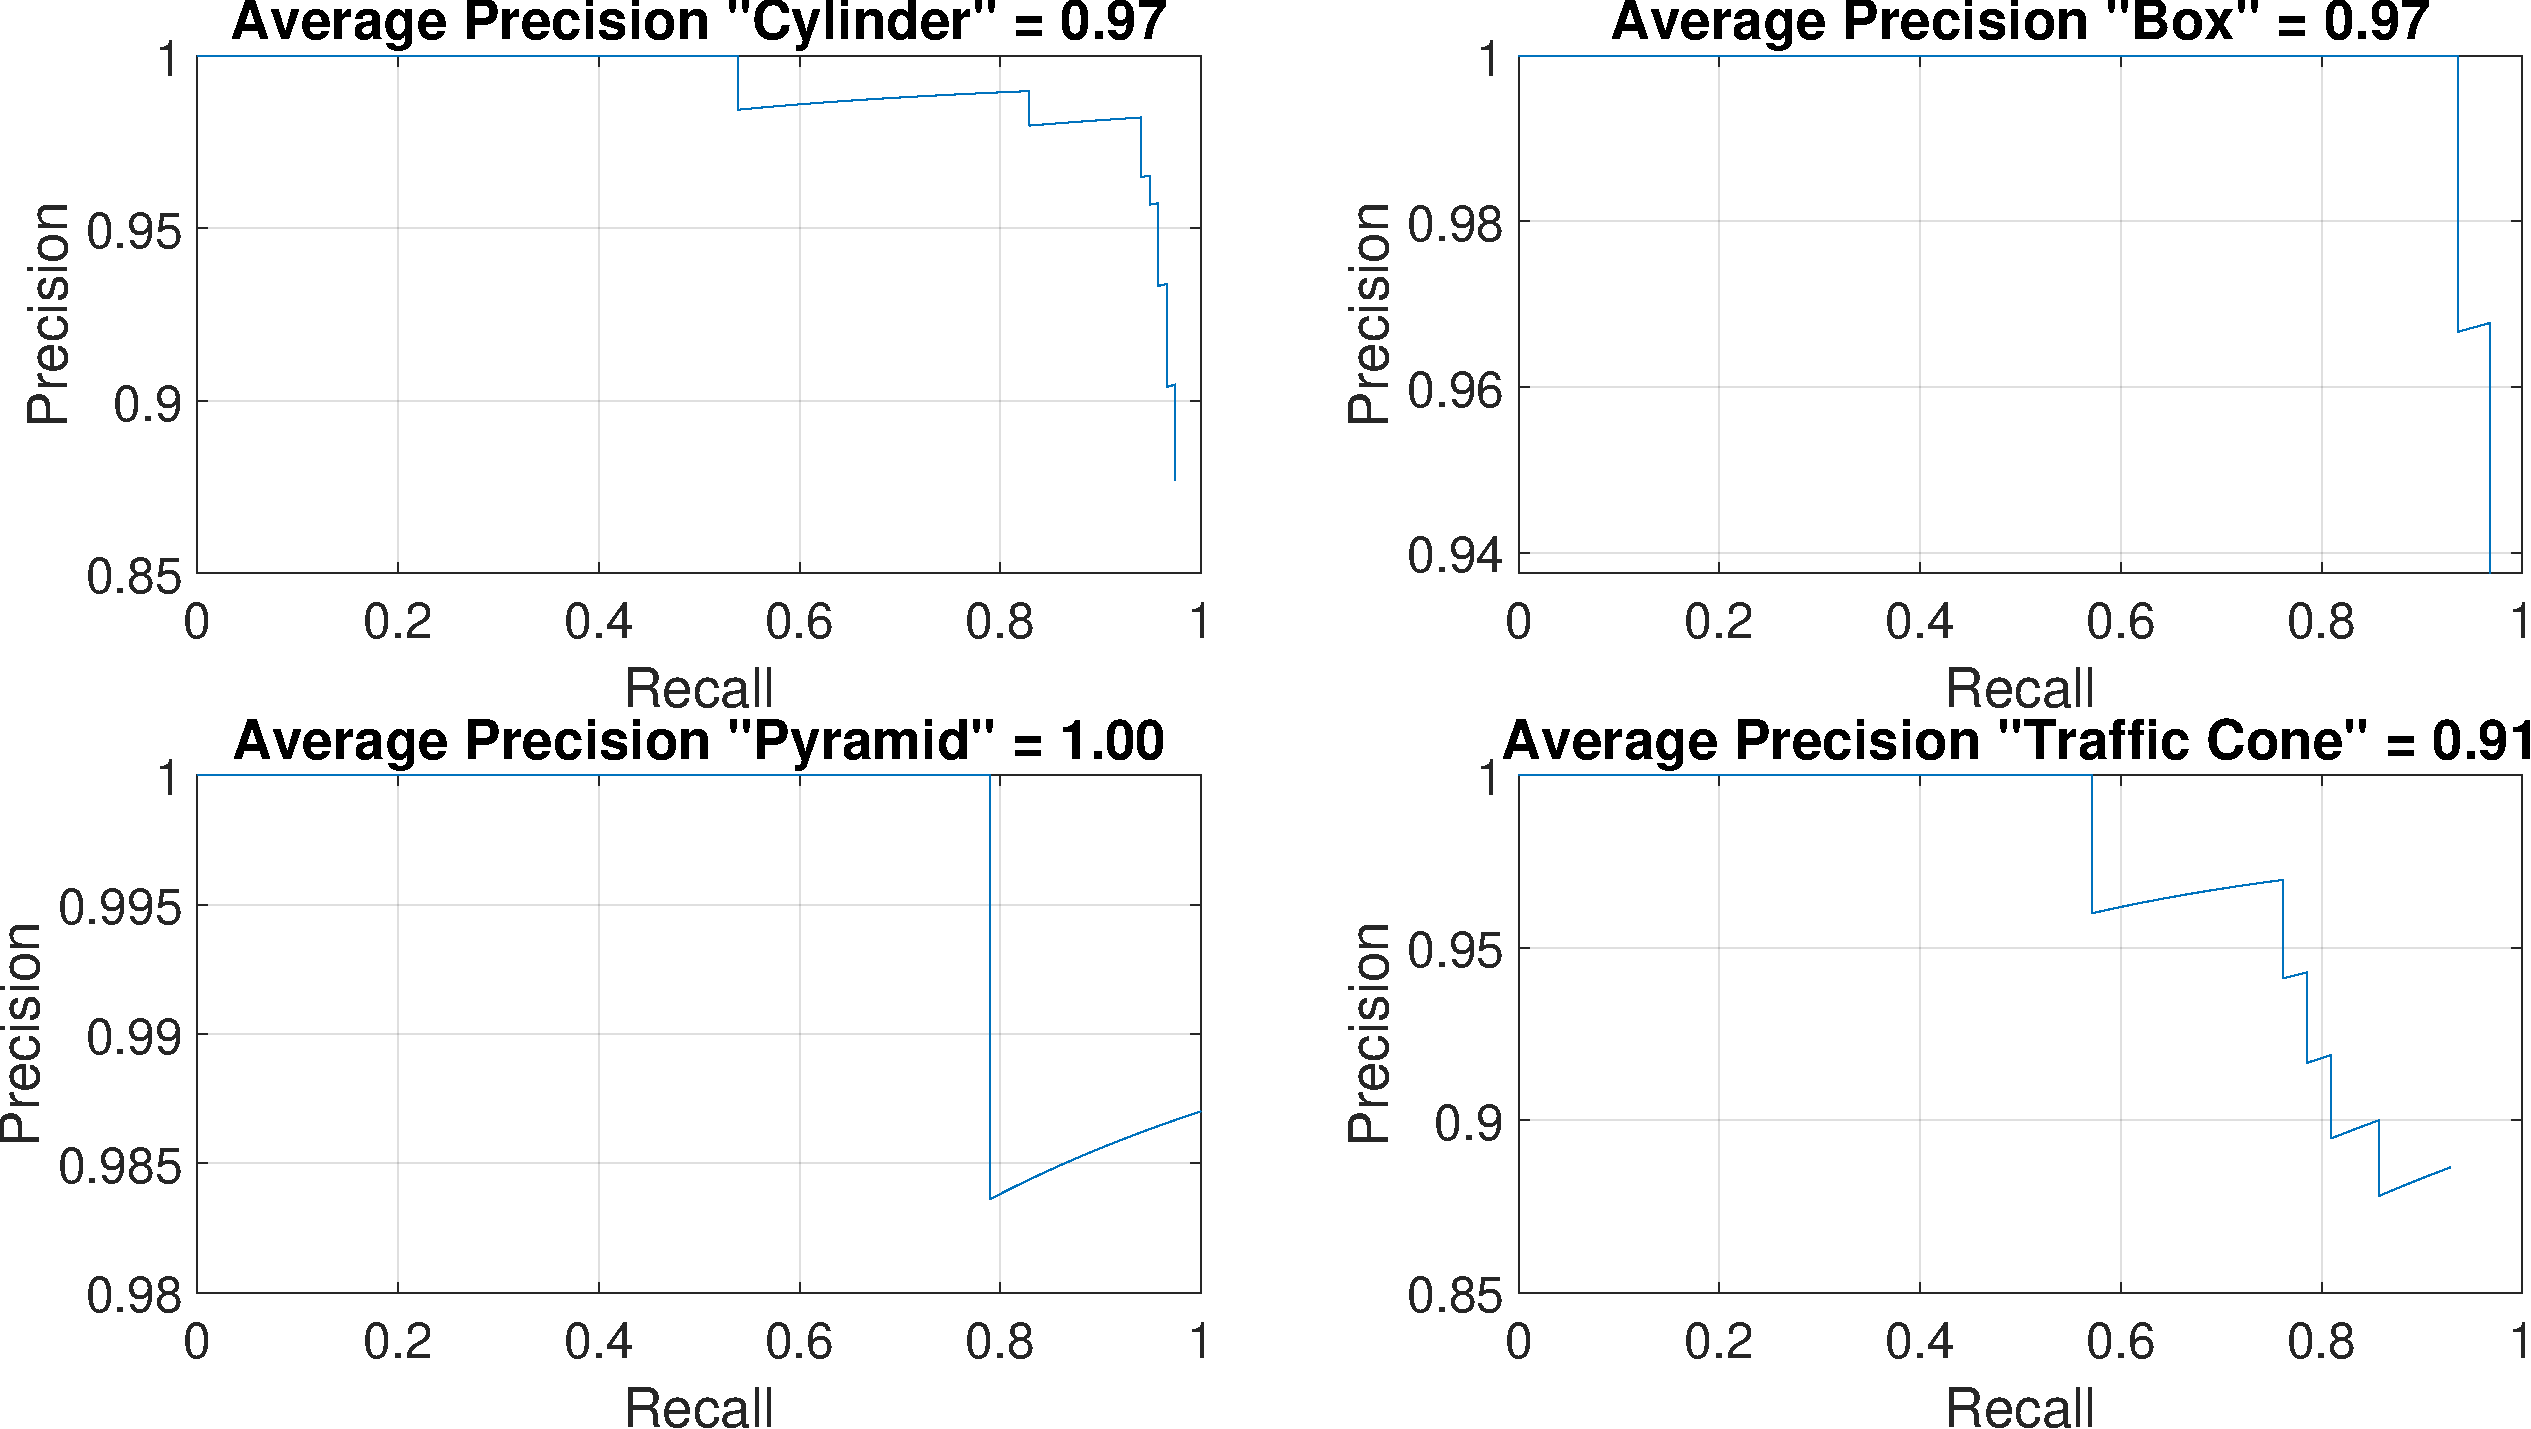
\includegraphics[width=0.9\textwidth]{Images/Precision.pdf}
    \caption{Overall Precision of Test Batch}
    \label{Precision_plot}
\end{figure}

There is a small difference between testing and training accuracy as shown in Table \ref{testperformance}. It represents the network has a small variance during the training. Therefore,  it is inferred that the network over-fits on some outliers. However, the difference between test and train accuracy is not too large so such outliers do not degrade the network performance. Additionally, the mean IoU of the test data is 0.81, which shows the ability to accurately predict the bounding box to localize the objects within the frame. The overall precision for each class of object is shown in Fig. \ref{Precision_plot}. In the test period, the network seems to be robust, and the average processing time is 59 ms per frame. 

The confusion chart is shown in Fig.\ref{confusionchart} for the classification result of the test batch. The network can identify 91\% of the objects. The empty label on prediction axis represents that the object has a label in ground truth data but was not detected by the network; on the flip side, the empty label on the true classes axis states that the object does not have a label in ground truth data because it is partially visible in the frame but it was detected by the network. However, it can be noted that the trained network has never done the incorrect classification during the testing.

\begin{table}[b]
    \centering
    \begin{tabular}{|c|c|}
        \hline
        \textbf{Parameter} & \textbf{Worth} \\
        \hline
        Average Detection Time & 59 ms\\
        \hline
        mean IoU & 0.8157\\
        \hline
        Training Accuracy & 99.08\% \\
        \hline
        Testing Accuracy & 96.25\% \\
        \hline  
    \end{tabular}
    \caption{Performance Parameters of Testing}
    \label{testperformance}
\end{table}

\begin{figure}
    \centering
    \begin{subfigure}[]
        \centering
        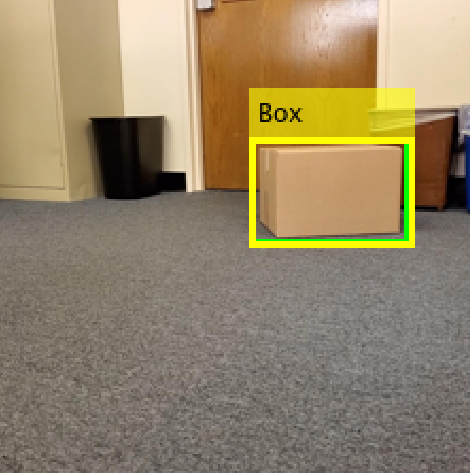
\includegraphics[width=0.38\textwidth]{Images/tt1.png}
    \end{subfigure}
    \begin{subfigure}[]
        \centering
        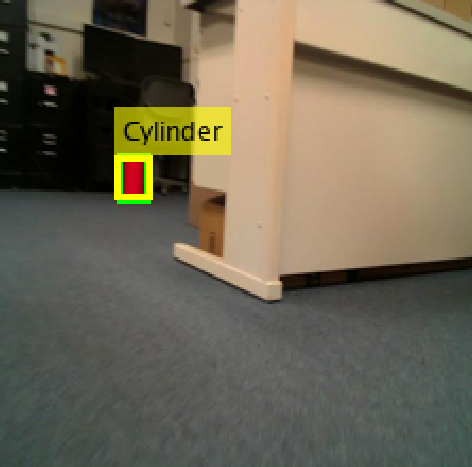
\includegraphics[width=0.38\textwidth]{Images/tt2.png}
    \end{subfigure}
    \begin{subfigure}[]
        \centering
        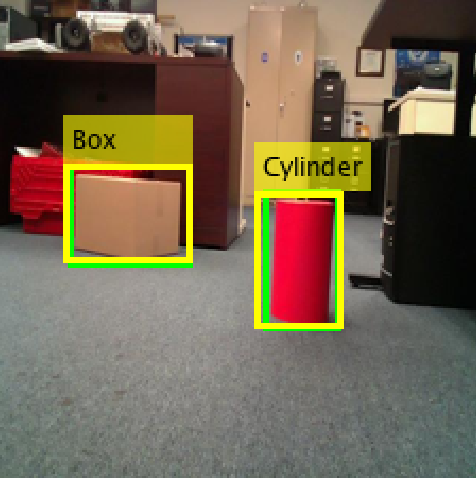
\includegraphics[width=0.38\textwidth]{Images/tt3.png}
    \end{subfigure}
    \begin{subfigure}[]
        \centering
        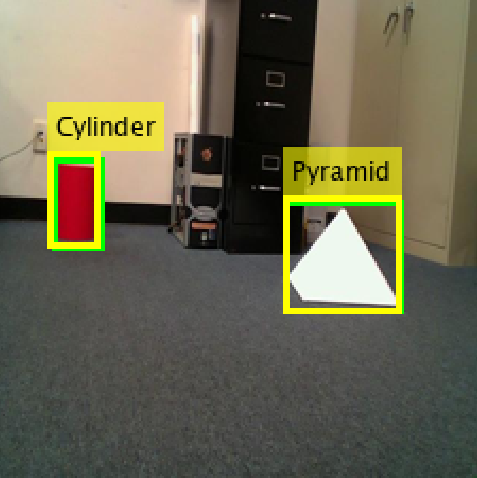
\includegraphics[width=0.38\textwidth]{Images/tt4.png}
    \end{subfigure}
    \begin{subfigure}[]
        \centering
        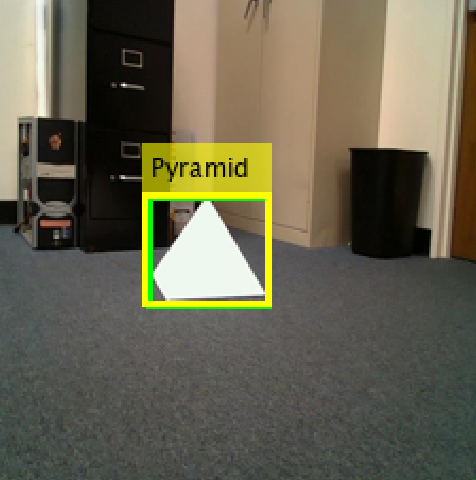
\includegraphics[width=0.38\textwidth]{Images/tt5.png}
    \end{subfigure}
    \begin{subfigure}[]
        \centering
        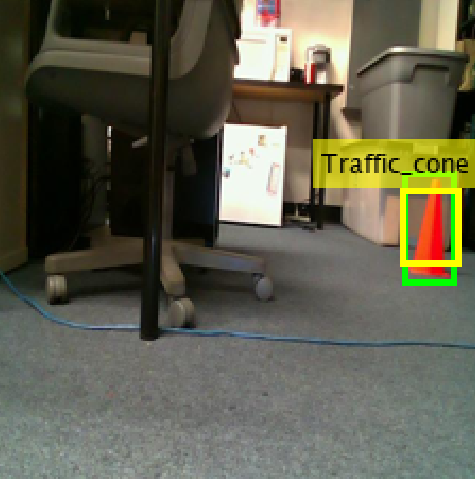
\includegraphics[width=0.38\textwidth]{Images/tt6.png}
    \end{subfigure}    
    \caption{True Positive Detections of Test Batch}
    \label{testdetection}
\end{figure}

\begin{table}[b]
    \centering
    \begin{tabular}{|c|c|c|c|c|}
        \hline
        \textbf{Image Tag} & \textbf{Object} & \textbf{Overlap Ratio} & \textbf{Precision} & \textbf{time}\\
        \hline
        (a) & Box & 0.95 & 97\% & 91 ms\\
        \hline
        (b) & Cylinder & 0.76 & 96\% & 75 ms\\
        \hline
        (c) & Cylinder & 0.85 & 89\% & 120 ms\\
        \hline
        (c) & Box & 0.92 & 99\% & 120 ms\\
        \hline  
        (d) & Cylinder & 0.77 & 98\% & 58 ms\\
        \hline
        (d) & Pyramid & 0.94 & 99\% & 58 ms\\
        \hline
        (e) & Pyramid & 0.93 & 99\% & 120 ms\\
        \hline 
        (f) & Traffic Cone & 0.62 & 99\% & 66 ms\\
        \hline
    \end{tabular}
    \caption{Performance Parameters of Detections in Fig.\ref{testdetection}}
    \label{tdp}
\end{table}

\begin{figure}
    \centering
    \begin{subfigure}[]
        \centering
        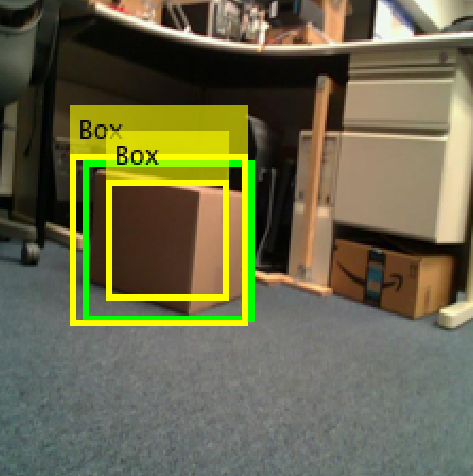
\includegraphics[width=0.38\textwidth]{Images/ft1.png}
    \end{subfigure}
    \begin{subfigure}[]
        \centering
        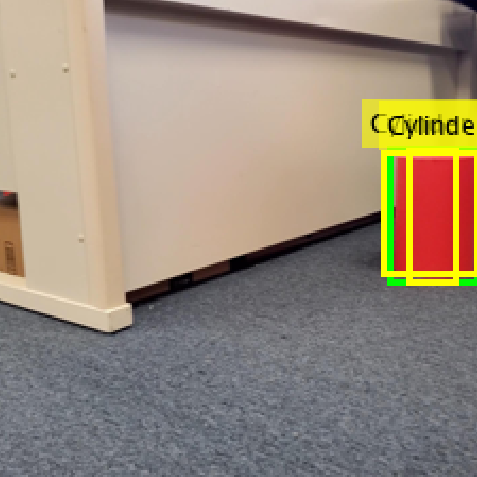
\includegraphics[width=0.38\textwidth]{Images/ft2.png}
    \end{subfigure}
    \begin{subfigure}[]
        \centering
        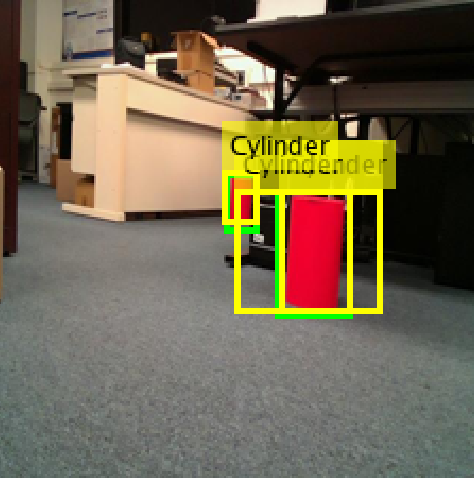
\includegraphics[width=0.38\textwidth]{Images/ft3.png}
    \end{subfigure}
    \begin{subfigure}[]
        \centering
        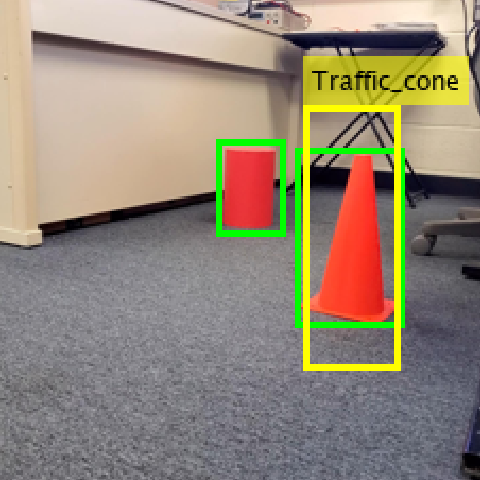
\includegraphics[width=0.38\textwidth]{Images/ft4.png}
    \end{subfigure}
    \begin{subfigure}[]
        \centering
        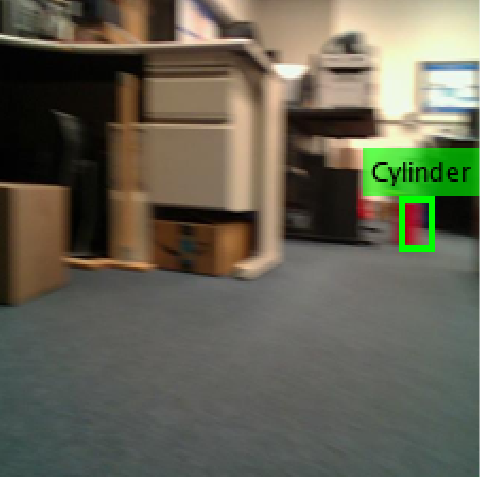
\includegraphics[width=0.38\textwidth]{Images/ft5.png}
    \end{subfigure}
    \begin{subfigure}[]
        \centering
        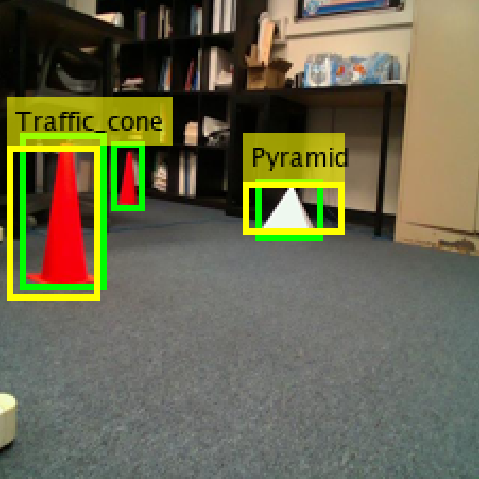
\includegraphics[width=0.38\textwidth]{Images/ft6.png}
    \end{subfigure}    
    \caption{Faulty Detections of Test Batch (a),(b), and (c) Multiple Detection for Single Object, (d) and (f) No Detection, and (e) No Detection due to Motion Blur}
    \label{faultydetection}
\end{figure}

\section{Real-time Object Detection Results and Position Estimation}

\begin{figure}[H]
    \centering
    \begin{subfigure}[]
        \centering
        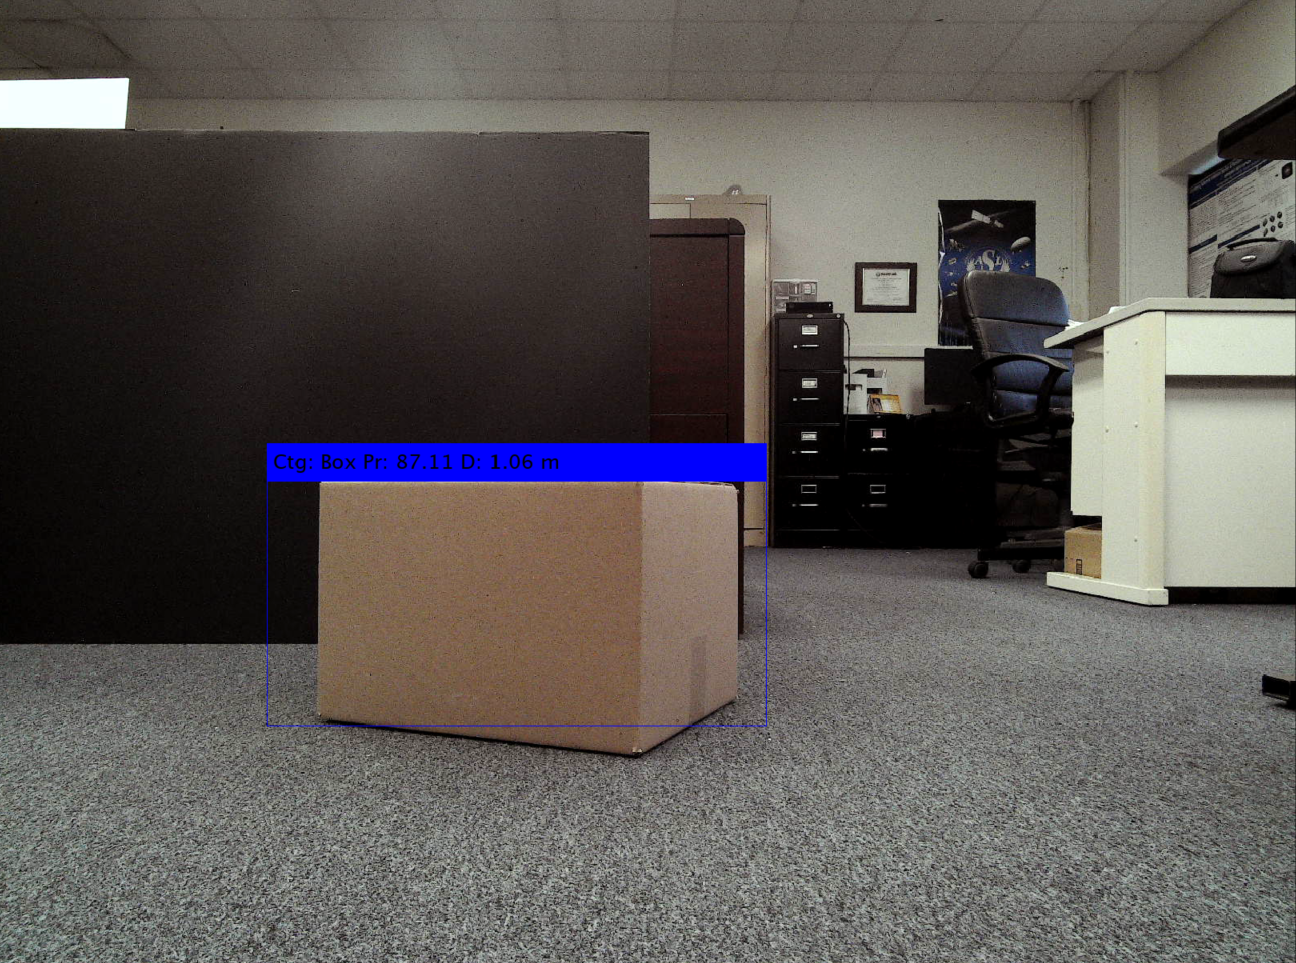
\includegraphics[width=0.45\textwidth]{Images/Box_d100cm.PNG}
    \end{subfigure}
    \begin{subfigure}[]
        \centering
        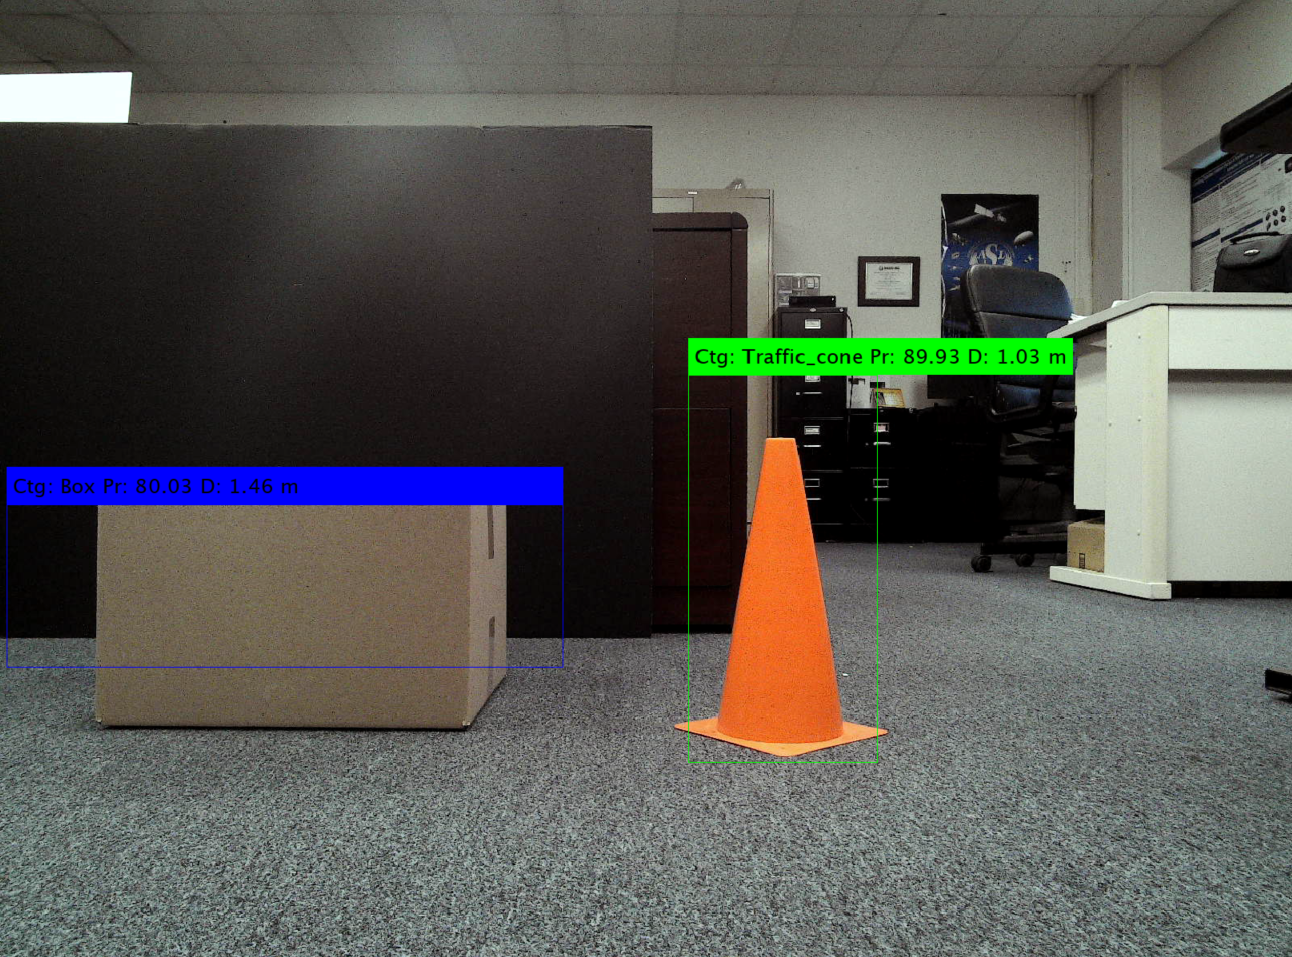
\includegraphics[width=0.45\textwidth]{Images/box_d120cm_py_d105cm.PNG}
    \end{subfigure}
    \begin{subfigure}[]
        \centering
        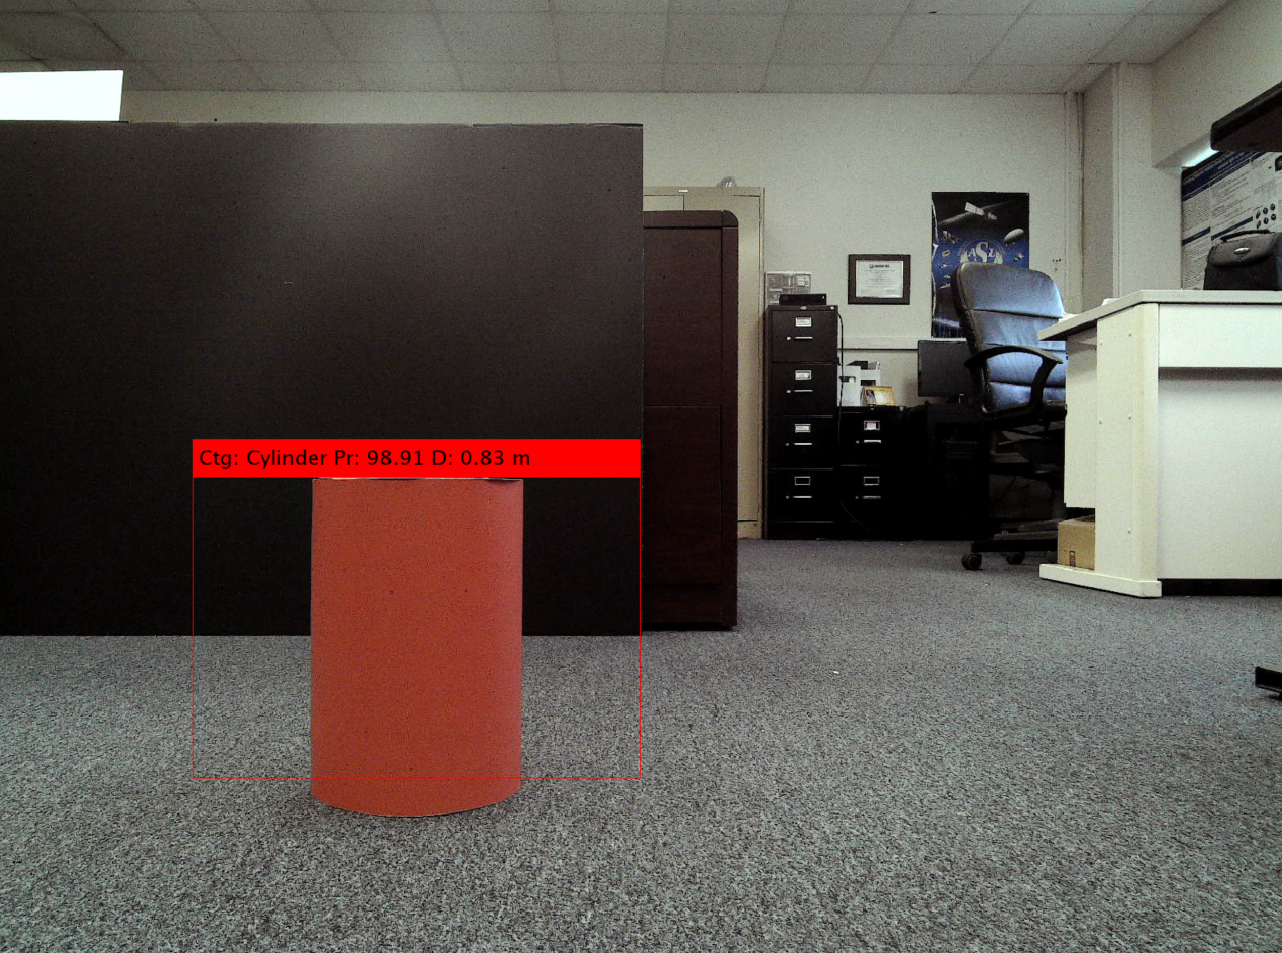
\includegraphics[width=0.45\textwidth]{Images/cy_d80cm.PNG}
    \end{subfigure}
    \begin{subfigure}[]
        \centering
        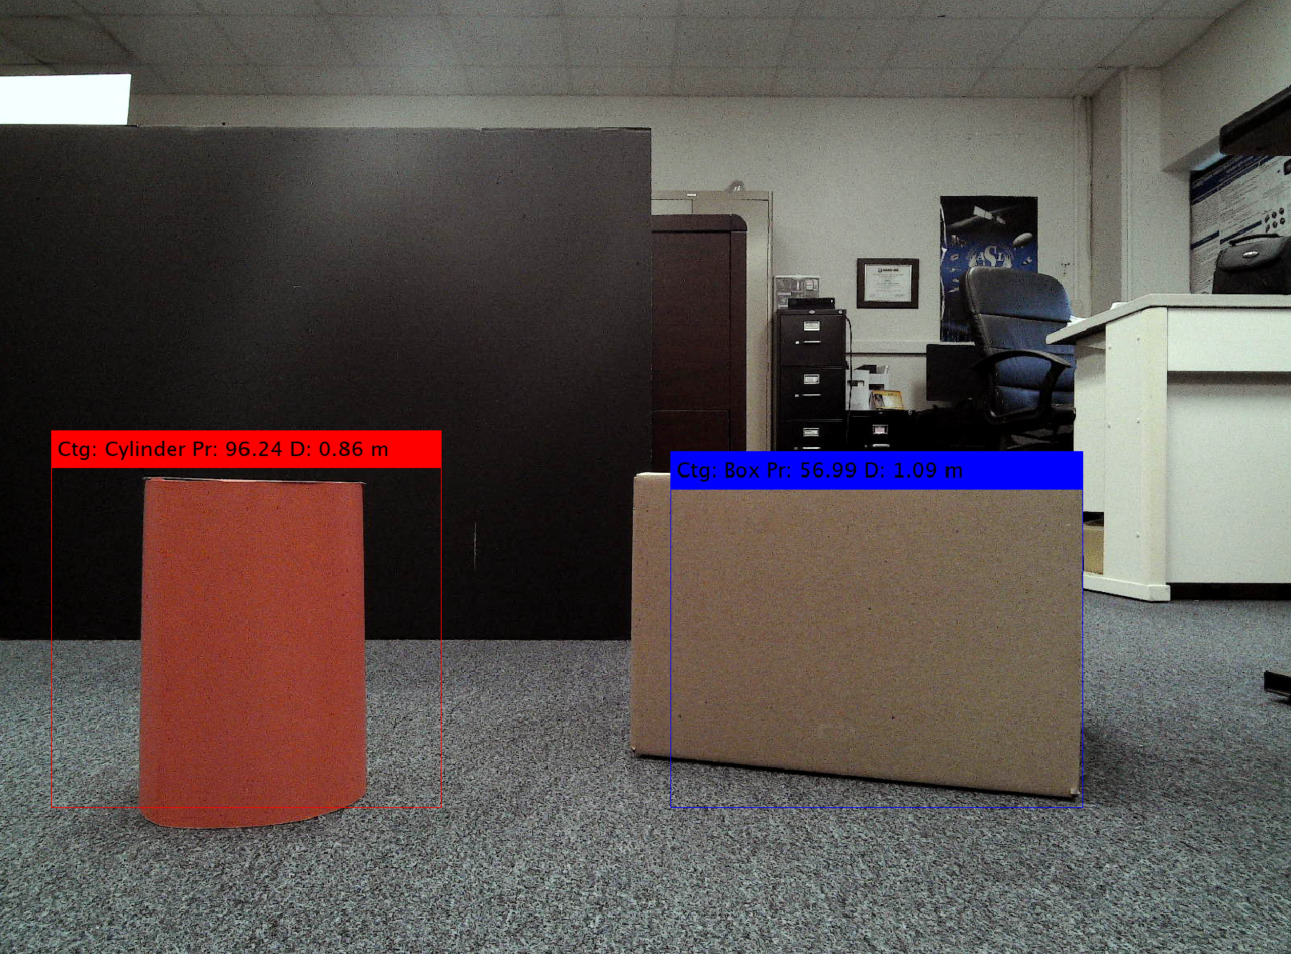
\includegraphics[width=0.45\textwidth]{Images/cy_d85cm_box_d95cm.PNG}
    \end{subfigure}
    \begin{subfigure}[]
        \centering
        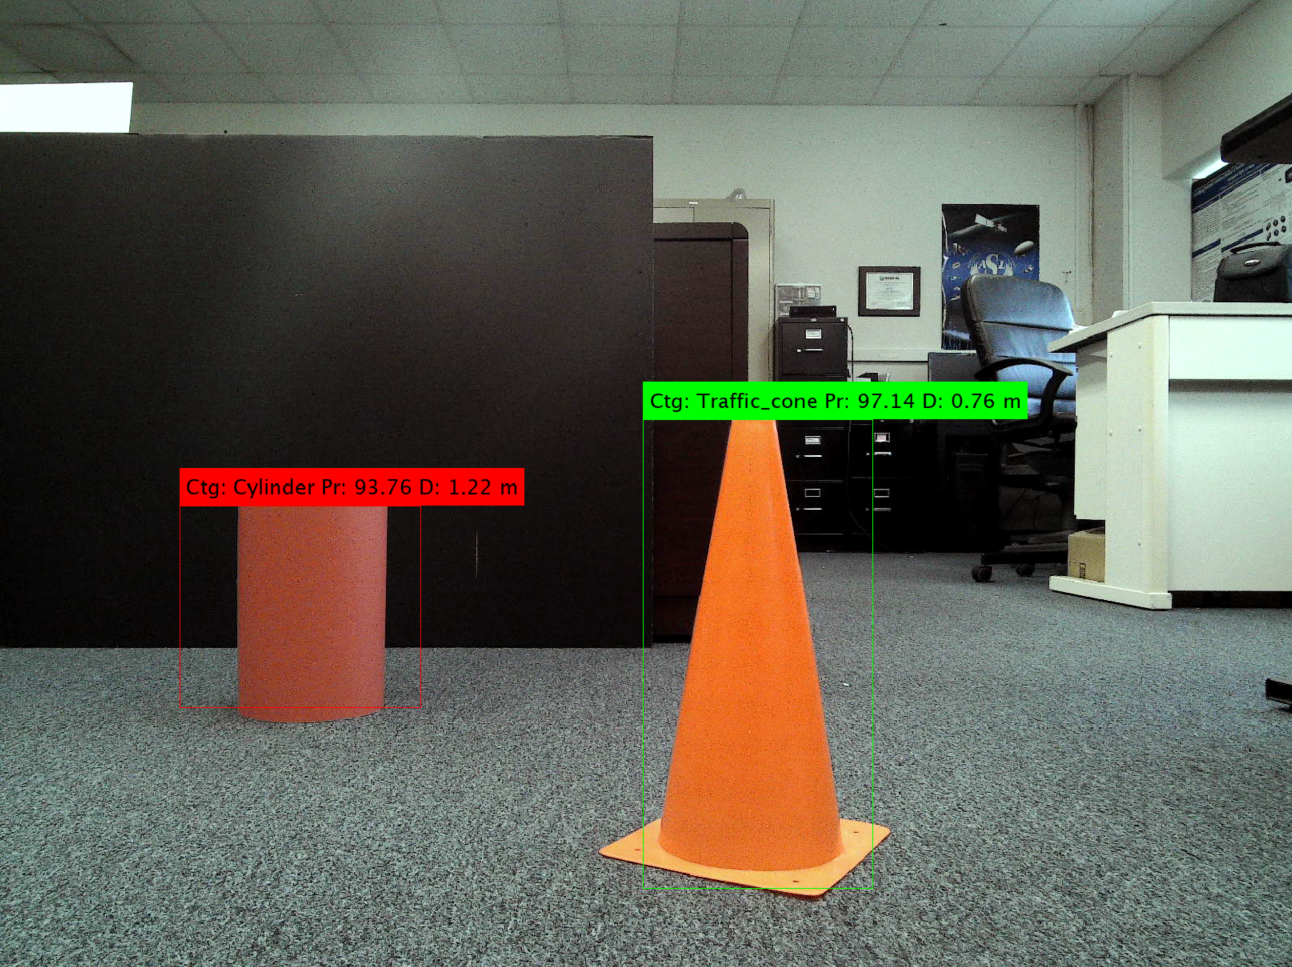
\includegraphics[width=0.45\textwidth]{Images/cy_d120cm_TC_d70cm.PNG}
    \end{subfigure}
    \begin{subfigure}[]
        \centering
        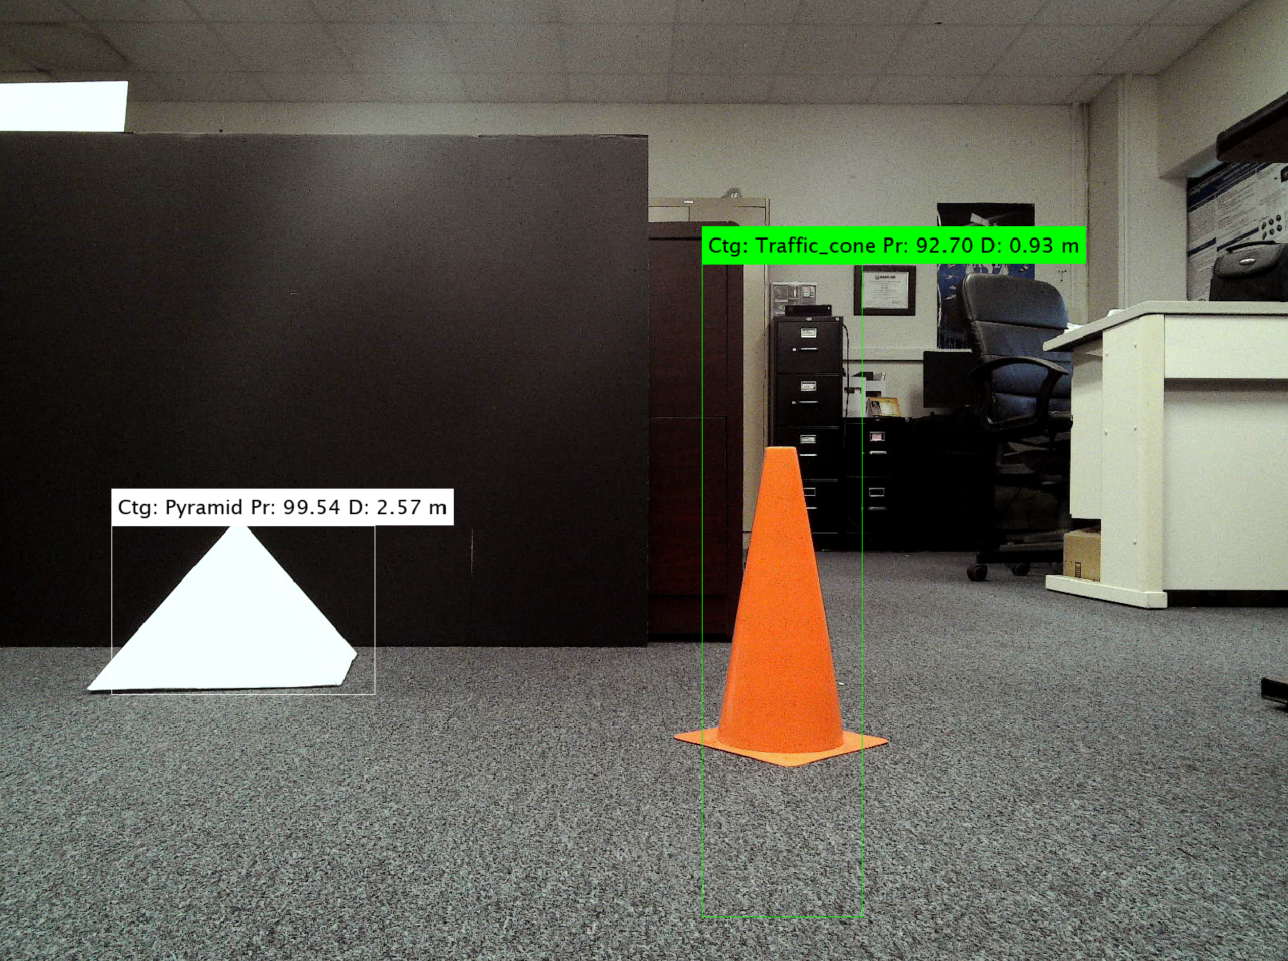
\includegraphics[width=0.45\textwidth]{Images/TC_d105cm_py_d155cm.PNG}
    \end{subfigure}    
    \caption{Real time Object Detection with Position Estimation}
    \label{realtimedetection}
\end{figure}


\section{Simulation Results of Sensor Fusion}
The simulation environment is created in MATLAB 2020b using the driving scene designer tool in order to evaluate the sensor fusion implementation. The essential parameters are defined as given in table \ref{paramsdrivingscene}. The lane, way-points, ego vehicle, object vehicle, and sensors definition are shown in Fig. \ref{Drivingscene}. The camera and LiDAR sensors are mounted on the ego vehicle and uncertainty in sensor measurements follows the white Gaussian noise. Since this sensor provides the measurement data w.r.t body frame of the ego vehicle, it does not require performing extrinsic calibration of a sensor to find the transformation matrix. Sensor's intrinsic calibration is performed from the measurement data and their standard measurement error is given in table \ref{sensorerrorscene}. The sensor covariance for LiDAR and camera which are derived from the calibration results are as follows. 

\begin{equation}
    R_{LiDAR} = 
    \left[\begin{array}{ccc}
    0.2102 & 0 & 0 \\
    0 & 0.0093 & 0 \\
    0 & 0 & 0.0001
    \end{array}\right] \\
\end{equation}

\begin{equation}
    R_{Camera} =
    \left[\begin{array}{ccc}
    1.5336 & 0 & 0 \\
    0 & 1.3365 & 0 \\
    0 & 0 & 0.0001
    \end{array}\right]
\end{equation}

Sensor fusion is implemented for the simulation environment using the linear Kalman filter. Dynamic model of the system is considered as a linear constant acceleration model. In order to characterize the performance of the sensor fusion, the estimated error is compared with sensor measurement error in table \ref{sensorerrorscene} and time history is shown in Fig. \ref{Residue_error_plot}. It is inferred that the estimation error is improved by 56\% compared to camera measurement error and reduction in variance after Camera-LiDAR fusion as shown in the residue error plot w.r.t in Fig. \ref{Residue_error_plot}. 

Moreover, the states which cannot be measured by sensors can be estimated through sensor fusion such as velocity and acceleration. In Fig. \ref{Stateestimation}, the time history of the estimated position, velocity, and acceleration is illustrated and compared with the available ground truth data.

\begin{figure}
    \centering
    \begin{subfigure}[]
        \centering
        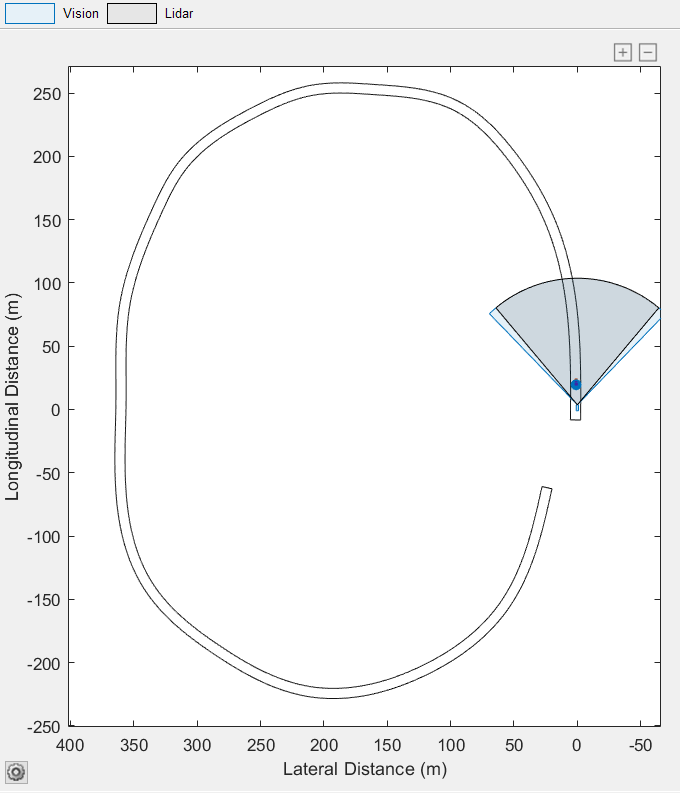
\includegraphics[width=0.4\textwidth]{Images/Drivingscene.png}
    \end{subfigure}
    \begin{subfigure}[]
        \centering
        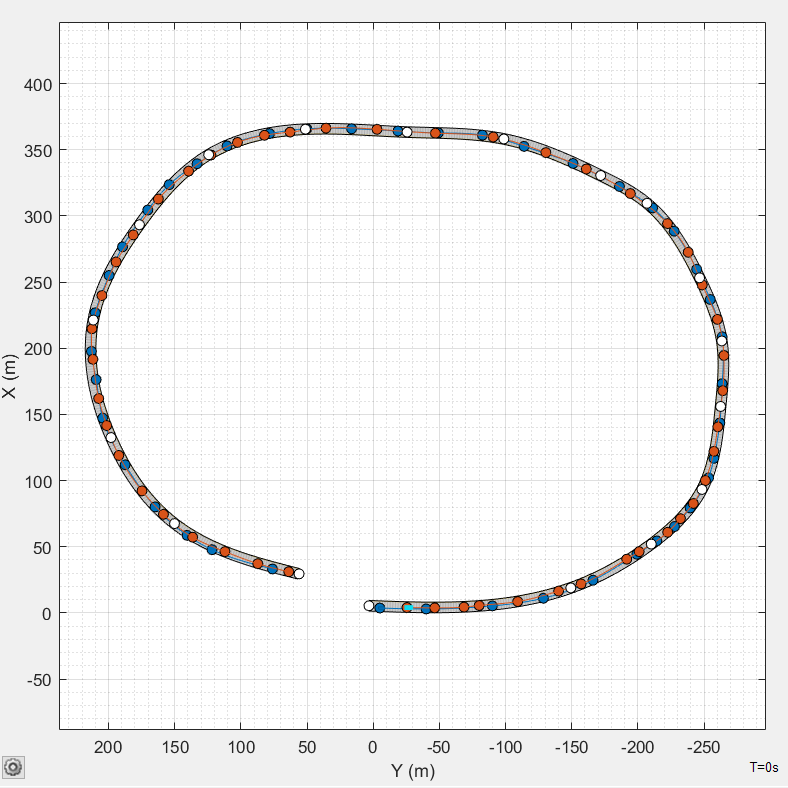
\includegraphics[width=0.47\textwidth]{Images/waypoints.png}
    \end{subfigure}
    \caption{Driving Scene in Simulation (a) Bird's Eye View of Scene (b) Way points Definition}
    \label{Drivingscene}
\end{figure}

\begin{table}
    \centering
    \begin{tabular}{|c|c|}
        \hline
        \textbf{Scene Parameter} & \textbf{Worth} \\
        \hline
        Ego Vehicle Speed & 30 m/s (67 mph)\\
        \hline
        Object Vehicle Speed & 30 m/s (67 mph)\\
        \hline
        Camera Azimuthal Limits & [-43 43] (deg) \\
        \hline
        Camera Elevation Limits & [-90 90] (deg)\\
        \hline  
        LiDAR Azimuthal Limits & [-40 40] (deg)\\
        \hline
        LiDAR Elevation Limits & [-90 90] (deg)\\
        \hline
    \end{tabular}
    \caption{Driving Scene Parameter Definitions}
    \label{paramsdrivingscene}
\end{table}

\begin{table}
    \centering
    \begin{tabular}{|c|c|c|c|}
        \hline
        \textbf{Description} & \textbf{Camera} & \textbf{LiDAR} & \textbf{Estimation} \\
        \hline
        X Error & 0.95 m & 0.29 m & 0.40 m\\
        \hline
        Y Error & 0.20 m & 0.033 m & 0.14 m\\
        \hline
        X Error & 0.0001 m & 0.0001 m & 0.00001 m\\
        \hline
        Overall Error & 0.97 m & 0.29 m & 0.42 m\\
        \hline        
    \end{tabular}
    \caption{Sensor Measurement and Residue Error in Driving Scene}
    \label{sensorerrorscene}
\end{table}

\begin{figure}
    \centering
    \begin{subfigure}
        \centering
        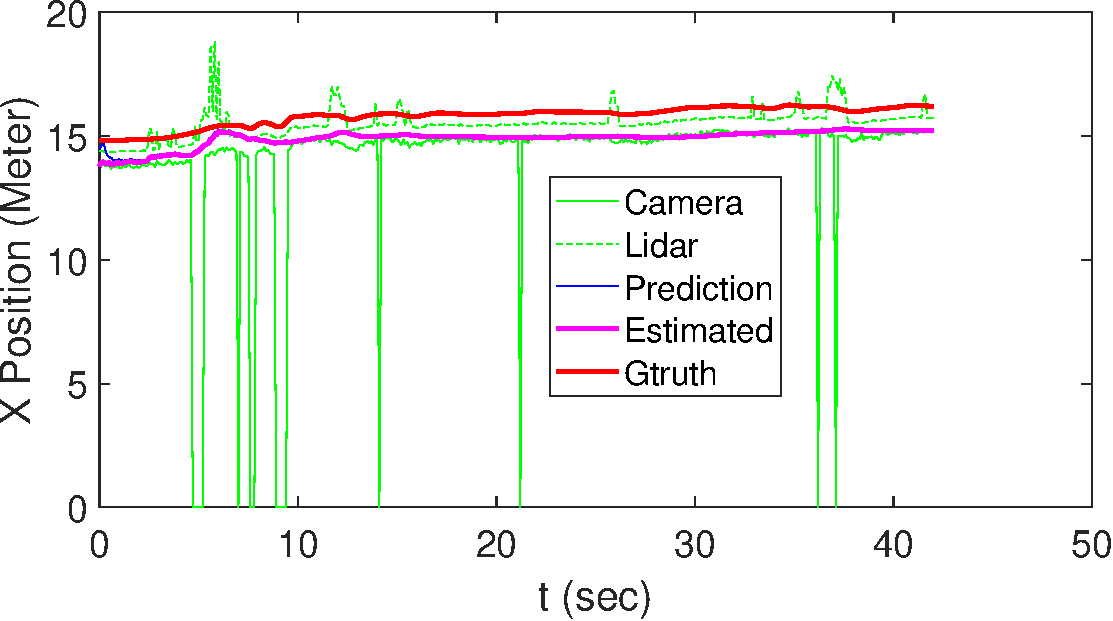
\includegraphics[height=6.5cm,width=0.9\textwidth]{Images/X_pos.pdf}
    \end{subfigure}
    \begin{subfigure}
        \centering
        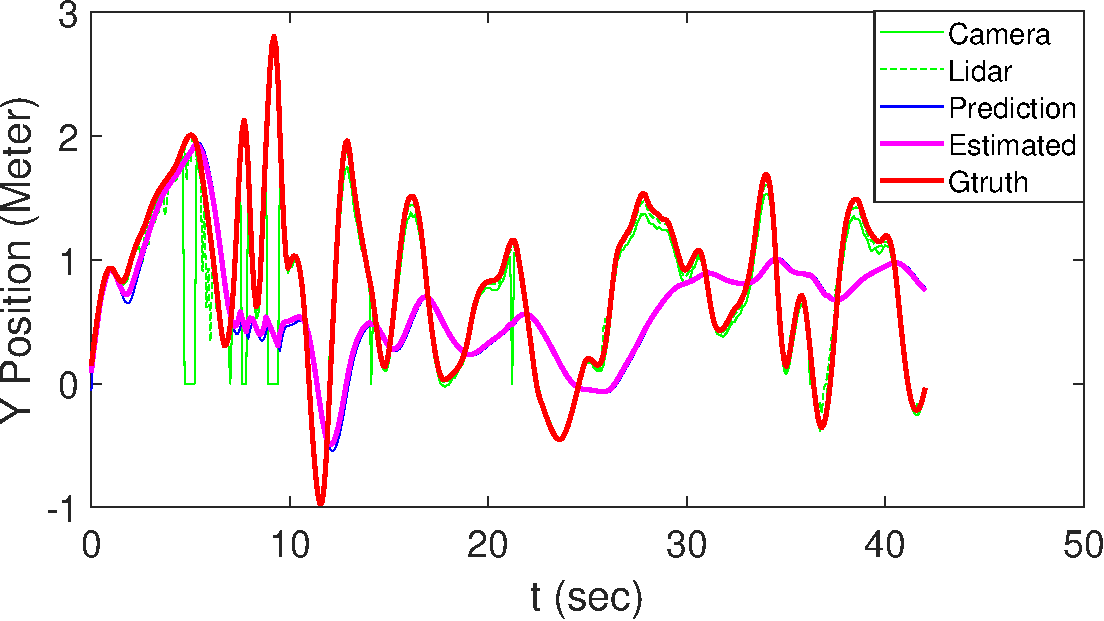
\includegraphics[height=6.5cm,width=0.9\textwidth]{Images/Y_pos.pdf}
    \end{subfigure}
    \begin{subfigure}
        \centering
        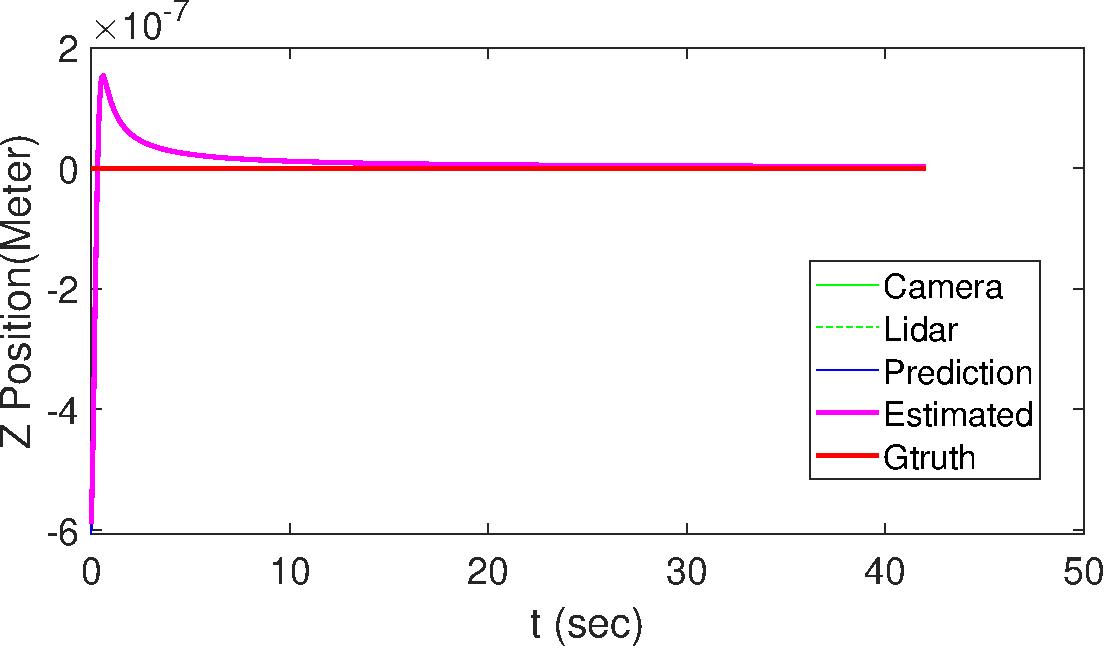
\includegraphics[height=6.5cm,width=0.9\textwidth]{Images/Z_pos.pdf}
    \end{subfigure}
    \caption{Position Estimation of Object in Simulation}
    \label{Stateestimation}
\end{figure}

\begin{figure}
    \centering
    \begin{subfigure}
        \centering
        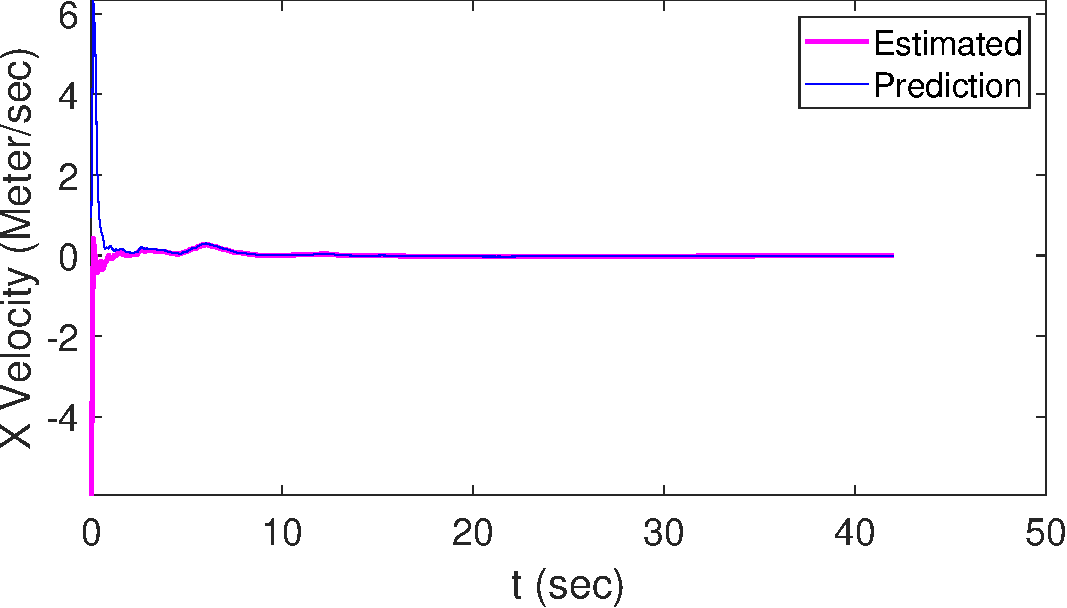
\includegraphics[height=6.5cm,width=0.9\textwidth]{Images/X_Vel.pdf}
    \end{subfigure}
    \begin{subfigure}
        \centering
        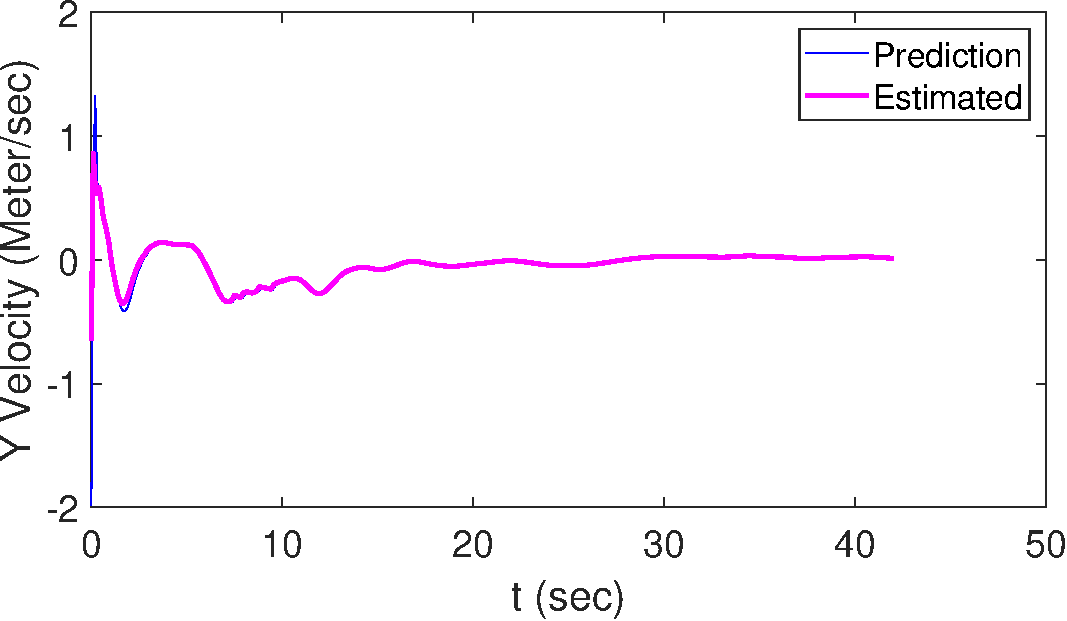
\includegraphics[height=6.5cm,width=0.9\textwidth]{Images/Y_Vel.pdf}
    \end{subfigure}
    \begin{subfigure}
        \centering
        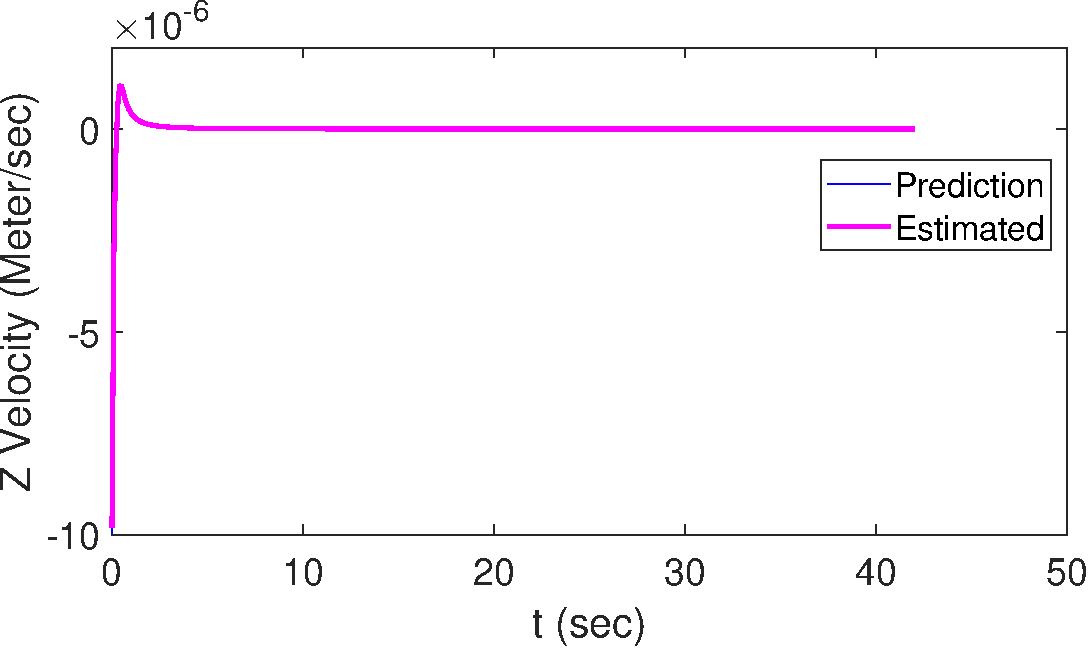
\includegraphics[height=6.5cm,width=0.9\textwidth]{Images/Z_Vel.pdf}
    \end{subfigure}
    \caption{Velocity Estimation of Object in Simulation}
    \label{Velestimation}
\end{figure}

\begin{figure}
    \centering
    \begin{subfigure}
        \centering
        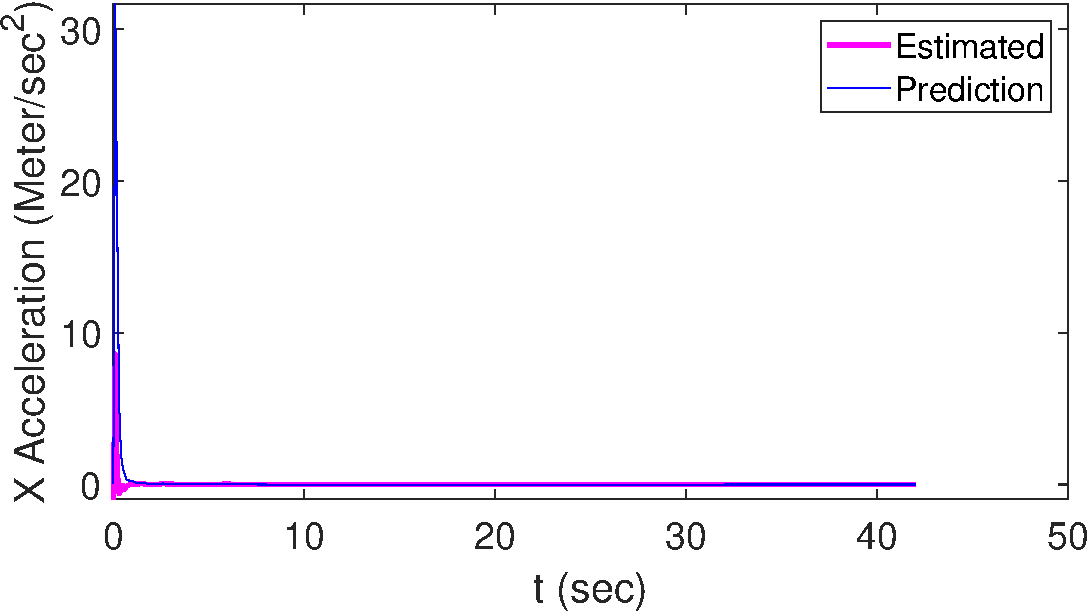
\includegraphics[height=6.5cm,width=0.9\textwidth]{Images/X_Acce.pdf}
    \end{subfigure}
    \begin{subfigure}
        \centering
        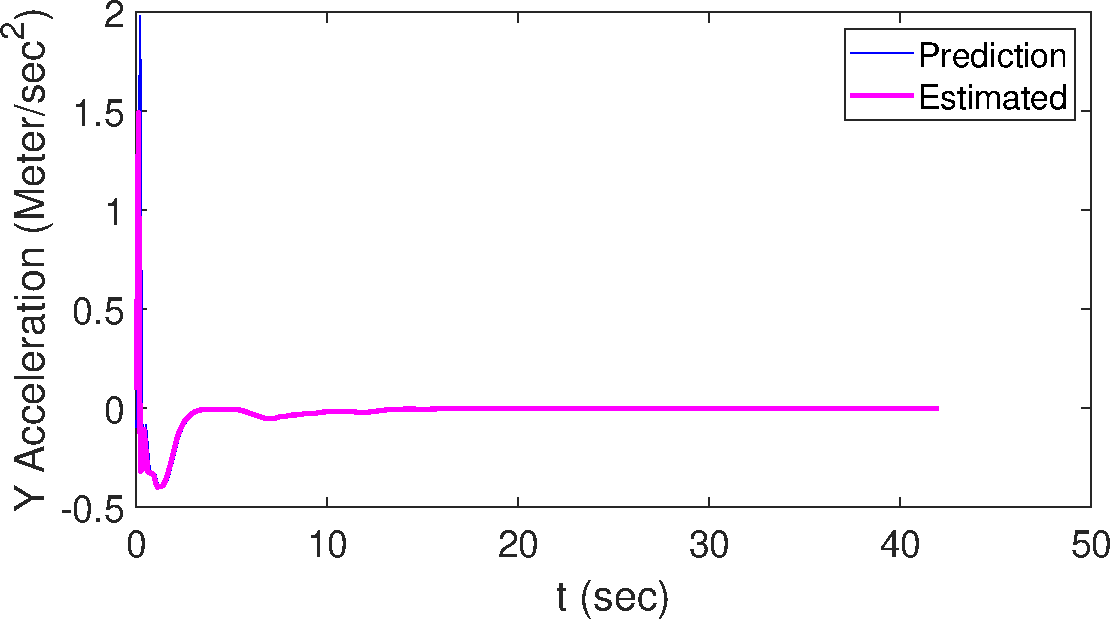
\includegraphics[height=6.5cm,width=0.9\textwidth]{Images/Y_Acce.pdf}
    \end{subfigure}
    \begin{subfigure}
        \centering
        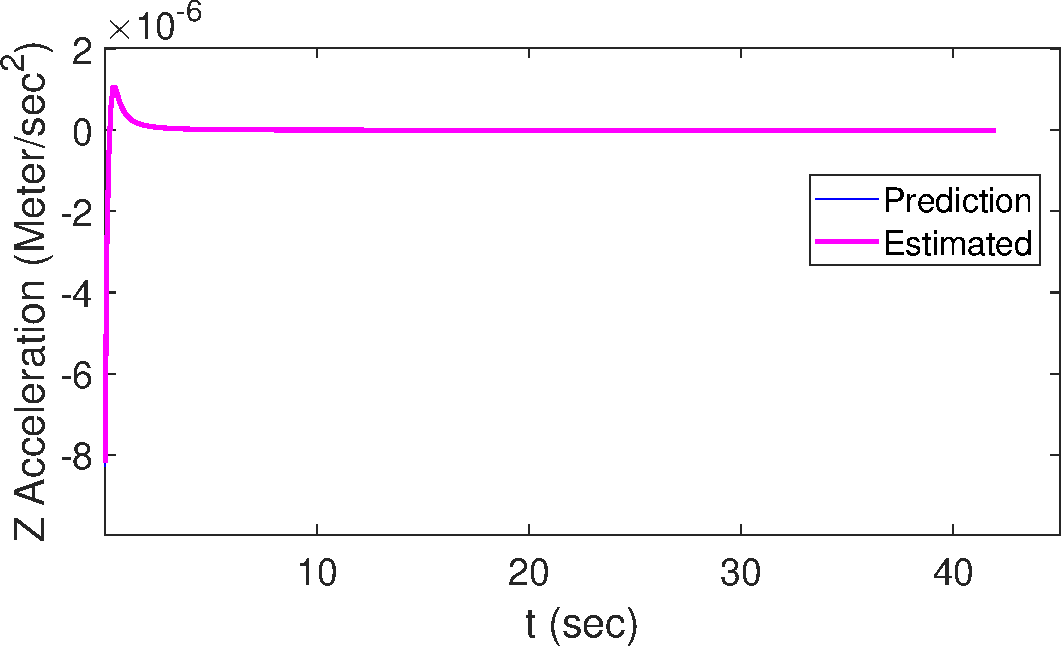
\includegraphics[height=6.5cm,width=0.9\textwidth]{Images/Z_Acce.pdf}
    \end{subfigure}
    \caption{Acceleration Estimation of Object in Simulation}
    \label{Accestimation}
\end{figure}


\begin{figure}
    \centering
    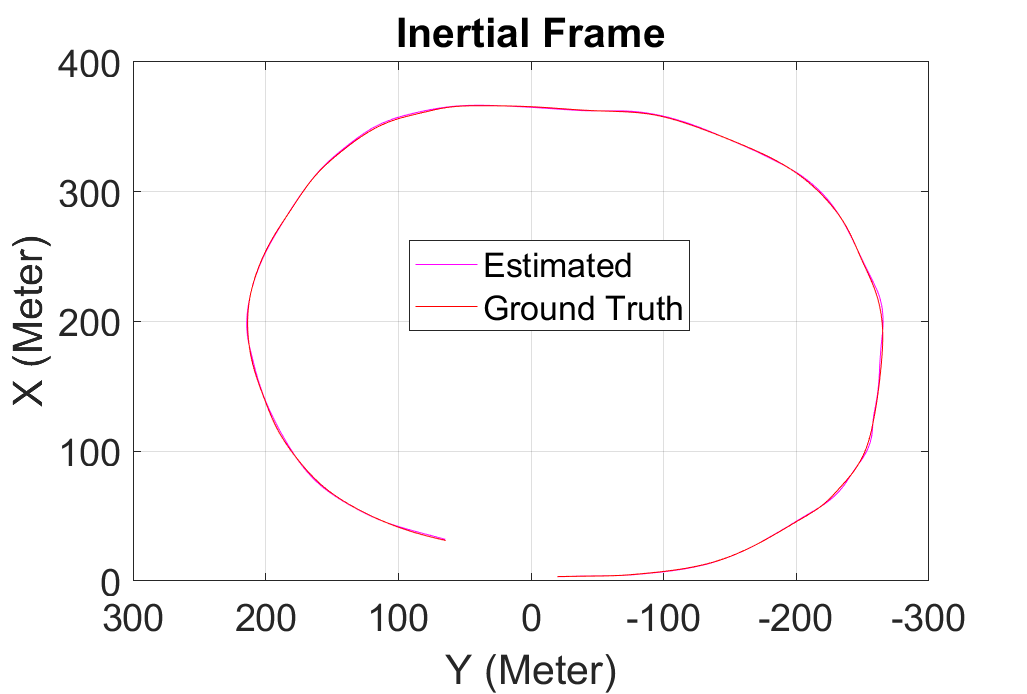
\includegraphics[width=0.9\textwidth]{Images/Trajectory.pdf}
    \caption{Trajectory Estimation of a Object w.r.t Inertial Frame}
    \label{Trajectory_plot}
\end{figure}   

\begin{figure}
    \centering
    \begin{subfigure}
        \centering
        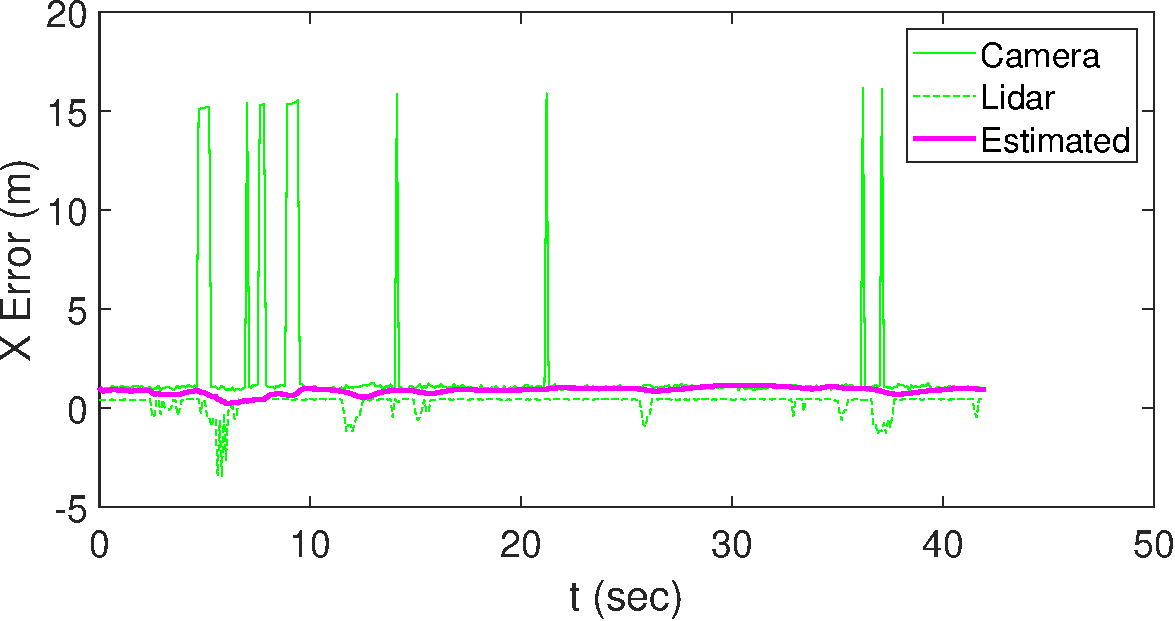
\includegraphics[height=6.5cm,width=0.9\textwidth]{Images/X_error.pdf}
    \end{subfigure}
    \begin{subfigure}
        \centering
        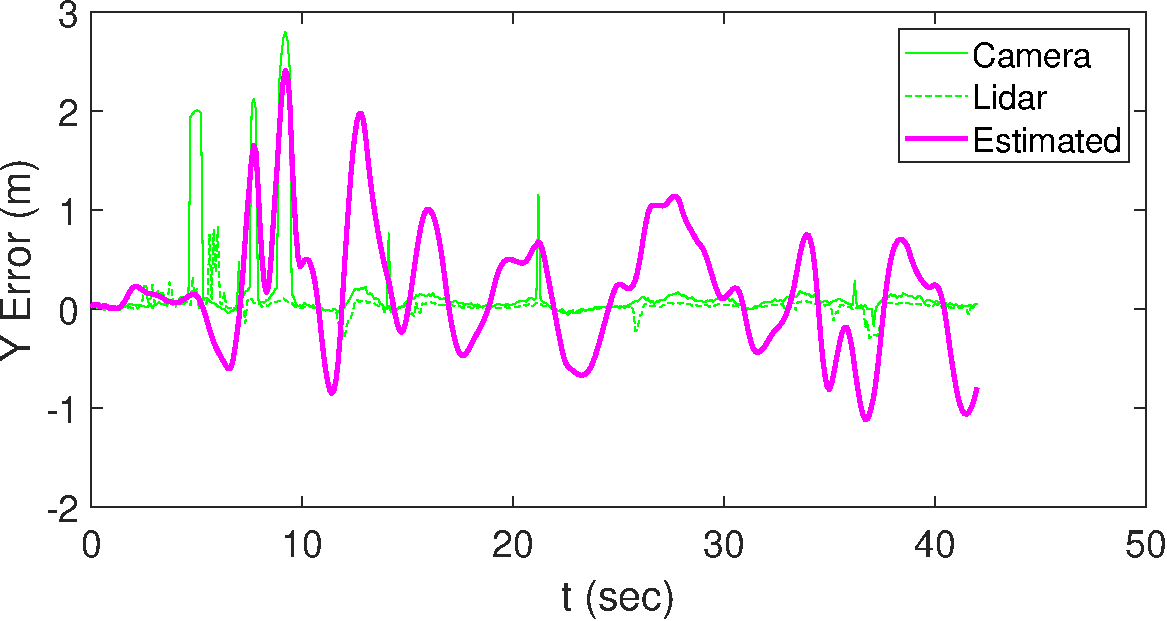
\includegraphics[height=6.5cm,width=0.9\textwidth]{Images/Y_error.pdf}
    \end{subfigure}
    \begin{subfigure}
        \centering
        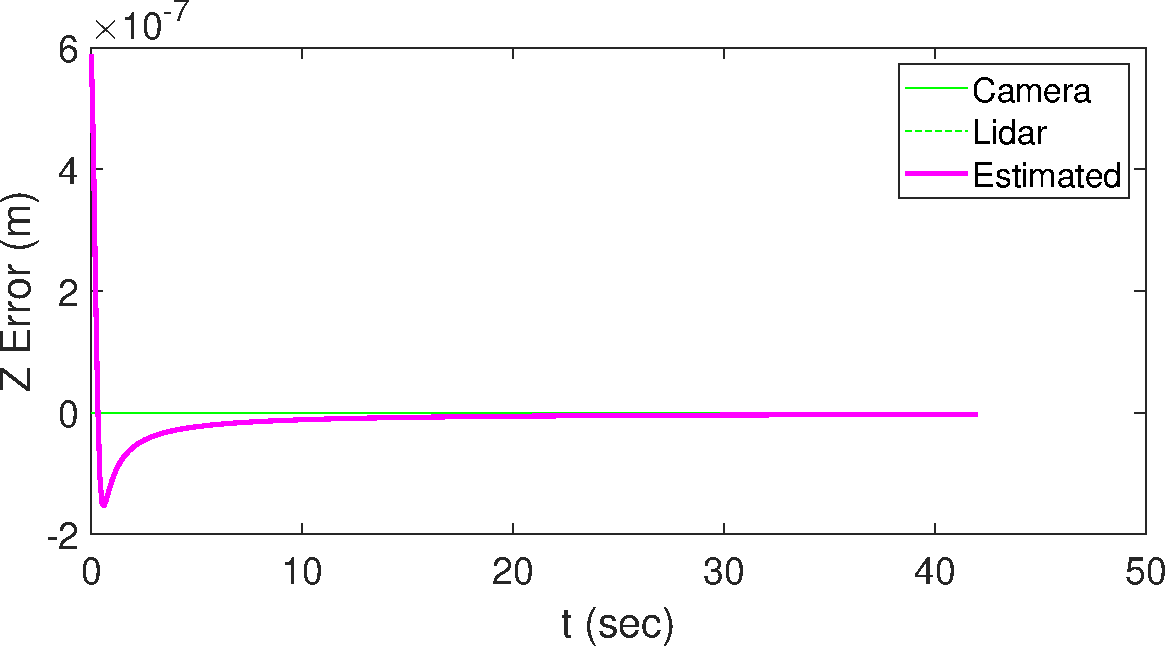
\includegraphics[height=6.5cm,width=0.9\textwidth]{Images/Z_error.pdf}
    \end{subfigure}
    \caption{Sensor Measurement and Estimation Error Plot}
    \label{Residue_error_plot}
\end{figure}


\section{Sensor Fusion Implementation on Hardware}
The real-time object estimation is implemented by fusing information from two optical sensors namely LiDAR and stereo camera. From the sensor intrinsic calibration, the sensor measurement covariance is derived for each sensor which is mention in Eq. (\ref{lidarcov}) and (\ref{cameracov}). The Linear Kalman filter is used to estimate the position of an object which we have discussed in the section \ref{linearkalmaanfilter}. Since the image label from the camera is used to predict the label from LiDAR data, both sensors are synchronized to generate measurement data at the same time. The data acquisition frequency for both synchronized sensors is 41 Hz. The NVIDIA GeForce GTX 1050 GPU is used to run the real-time object detection and position estimation framework. On this hardware, the average timestamp of 1.44 sec is achieved, unlike CPU based system that takes approximately 8 sec to completely process a single frame. 

The sensor fusion framework is used to estimate the position of an object detected by the YOLO-v3 network. The algorithm was tested for two objects Box and Traffic cone. Their position and velocity plots are shown in Fig. \ref{Stateestbox} and \ref{Stateesttc}. Moreover, the real-time object position estimation results are illustrated in Fig. \ref{realtimedetection}, and the label annotated on the bounding box shows the following information: Object category (Ctg), precision in detection (Pr), Estimated Distance from the vehicle (D), Estimated velocity w.r.t vehicle (V), and Estimated Acceleration w.r.t vehicle (a).

\vspace{5cm}
   
\begin{equation}
    R_{LiDAR} = 
    \left[\begin{array}{ccc}
    5.84e-05 & 0 & 0 \\
    0 & 2.73e-04 & 0 \\
    0 & 0 & 3.917e-06
    \end{array}\right] \\
    \label{lidarcov}
\end{equation}

\vspace{1cm}

\begin{equation}
    R_{Camera} =
    \left[\begin{array}{ccc}
    2.59e-05 & 0 & 0 \\
    0 & 9.76e-06 & 0 \\
    0 & 0 & 4.46e-04
    \end{array}\right]
    \label{cameracov}
\end{equation}

\begin{figure}
    \centering
    \begin{subfigure}
        \centering
        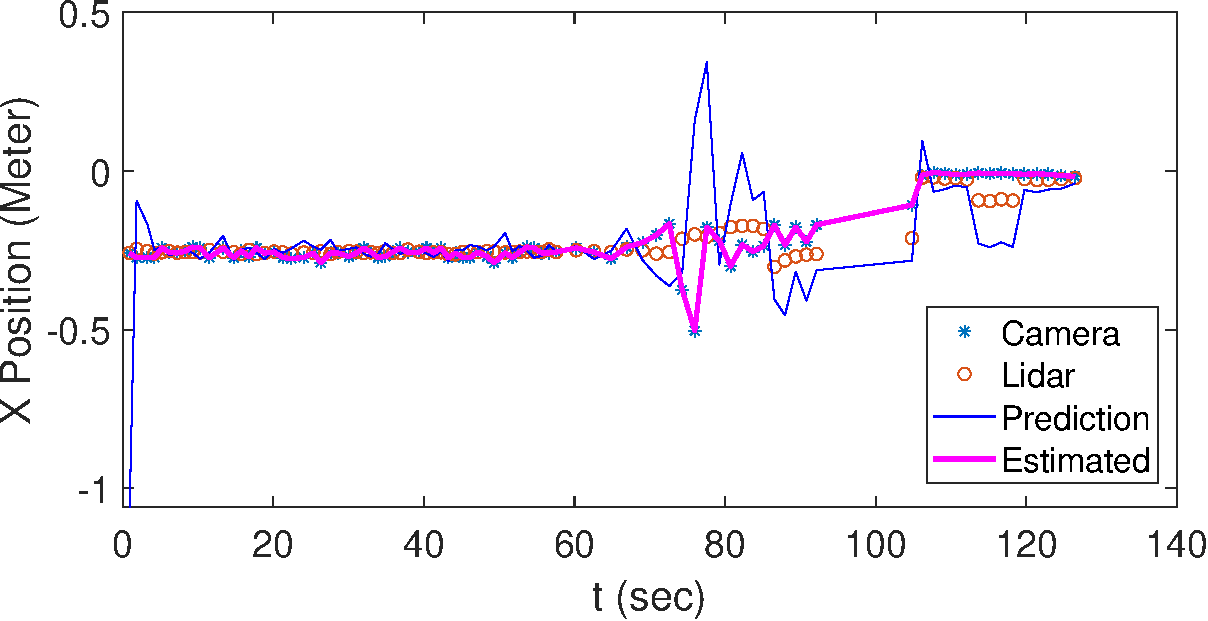
\includegraphics[height=6.5cm,width=0.9\textwidth]{Images/X_posbox.pdf}
    \end{subfigure}
    \begin{subfigure}
        \centering
        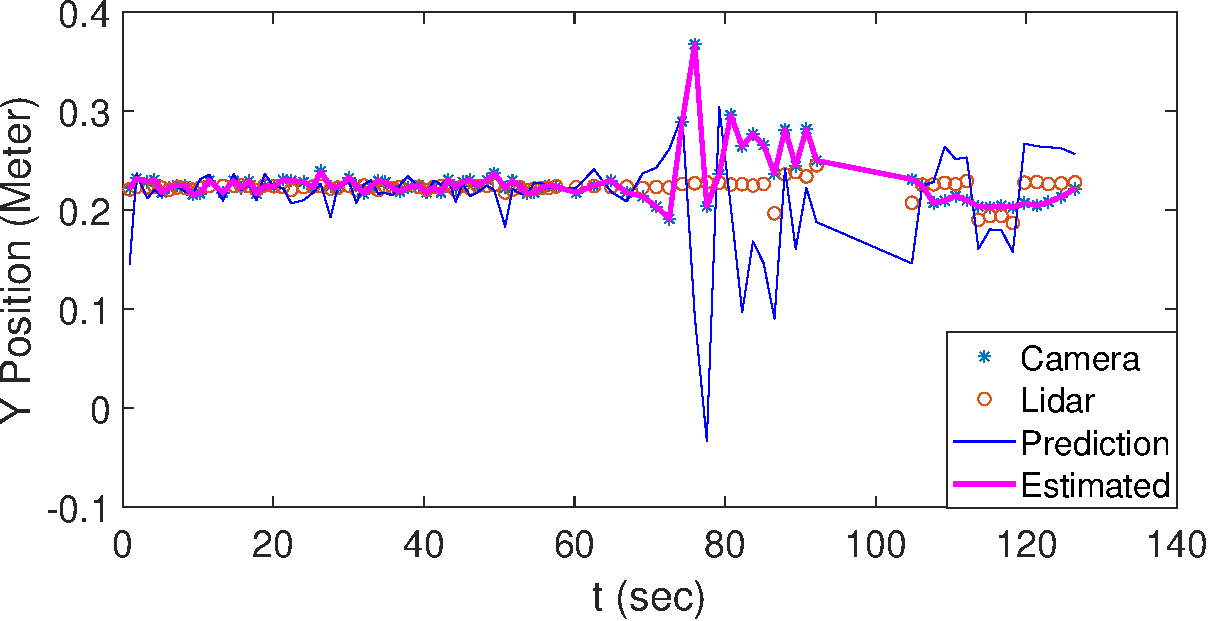
\includegraphics[height=6.5cm,width=0.9\textwidth]{Images/Y_posbox.pdf}
    \end{subfigure}
    \begin{subfigure}
        \centering
        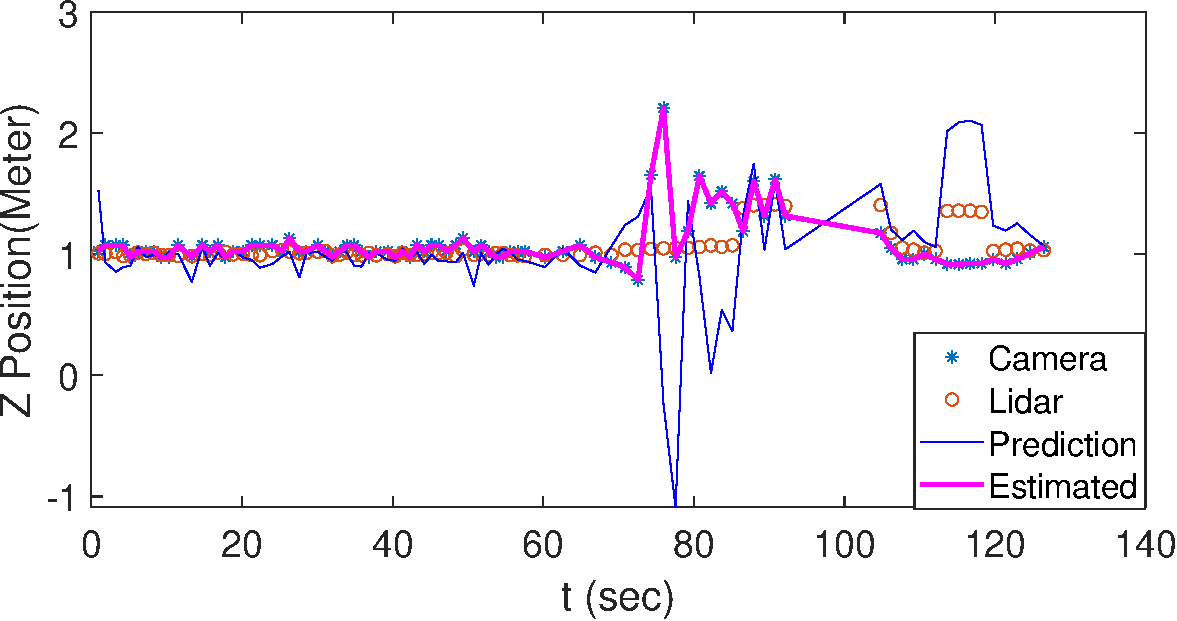
\includegraphics[height=6.5cm,width=0.9\textwidth]{Images/Z_posbox.pdf}
    \end{subfigure}
    \caption{Real time Position Estimation of a Object 'Box'}
    \label{Stateestbox}
\end{figure}

\begin{figure}
    \centering
    \begin{subfigure}
        \centering
        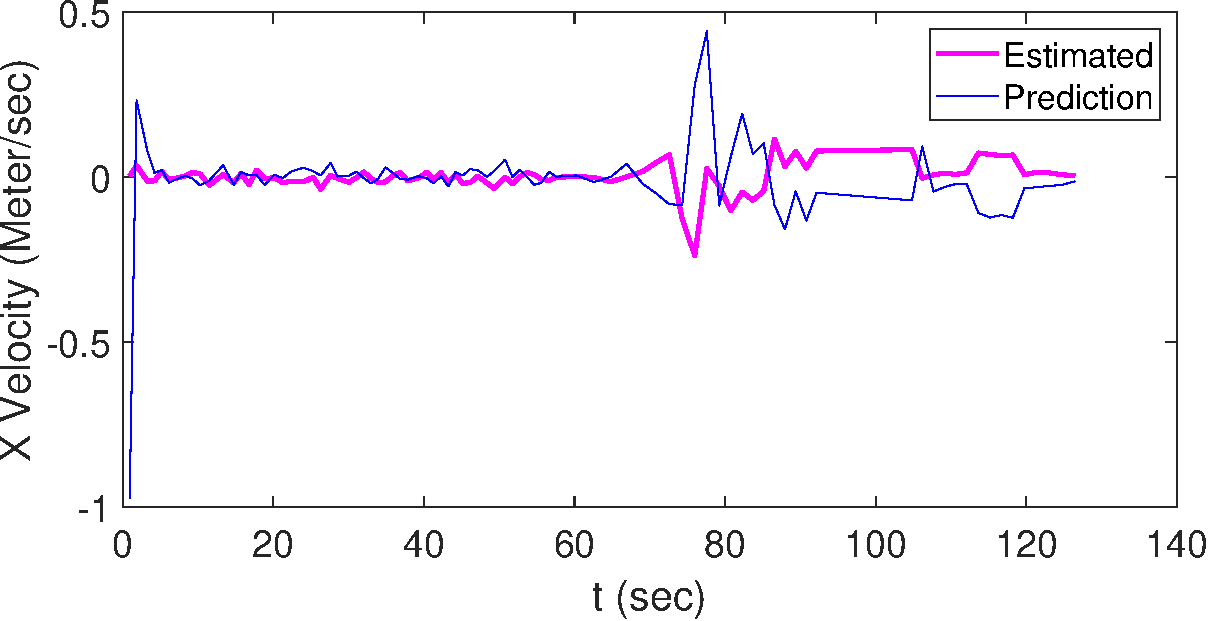
\includegraphics[height=6.5cm,width=0.9\textwidth]{Images/X_velbox.pdf}
    \end{subfigure}
    \begin{subfigure}
        \centering
        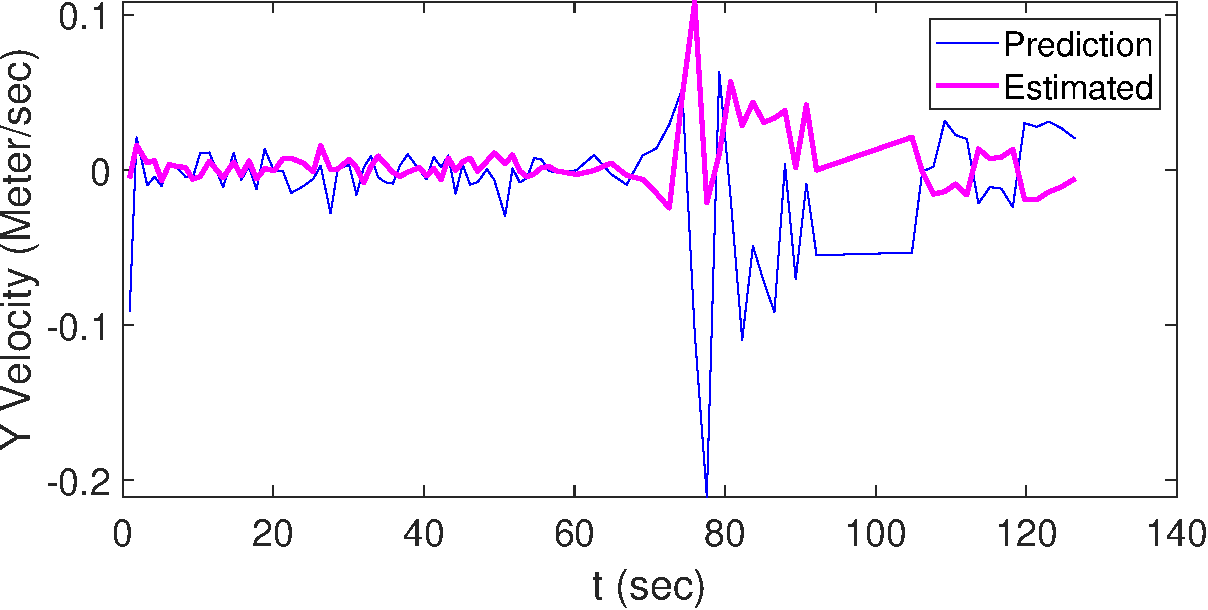
\includegraphics[height=6.5cm,width=0.9\textwidth]{Images/Y_velbox.pdf}
    \end{subfigure}
    \begin{subfigure}
        \centering
        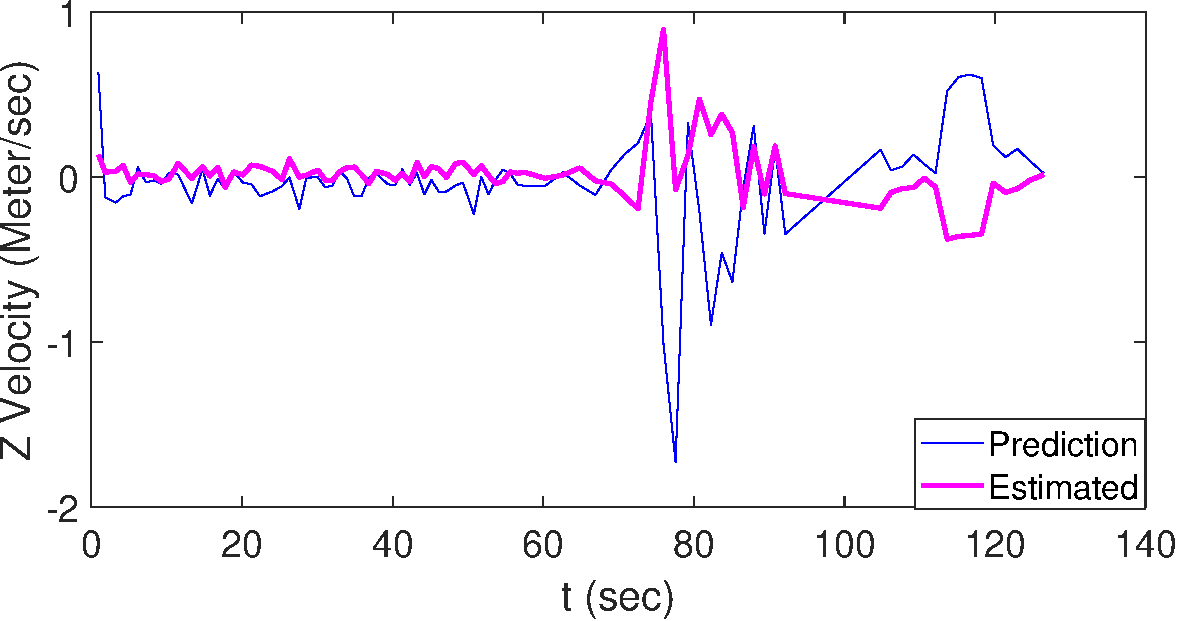
\includegraphics[height=6.5cm,width=0.9\textwidth]{Images/Z_velbox.pdf}
    \end{subfigure}
    \caption{Real time Velocity Estimation of a Object 'Box'}
    \label{Veloestbox}
\end{figure}

\begin{figure}
    \centering
    \begin{subfigure}
        \centering
        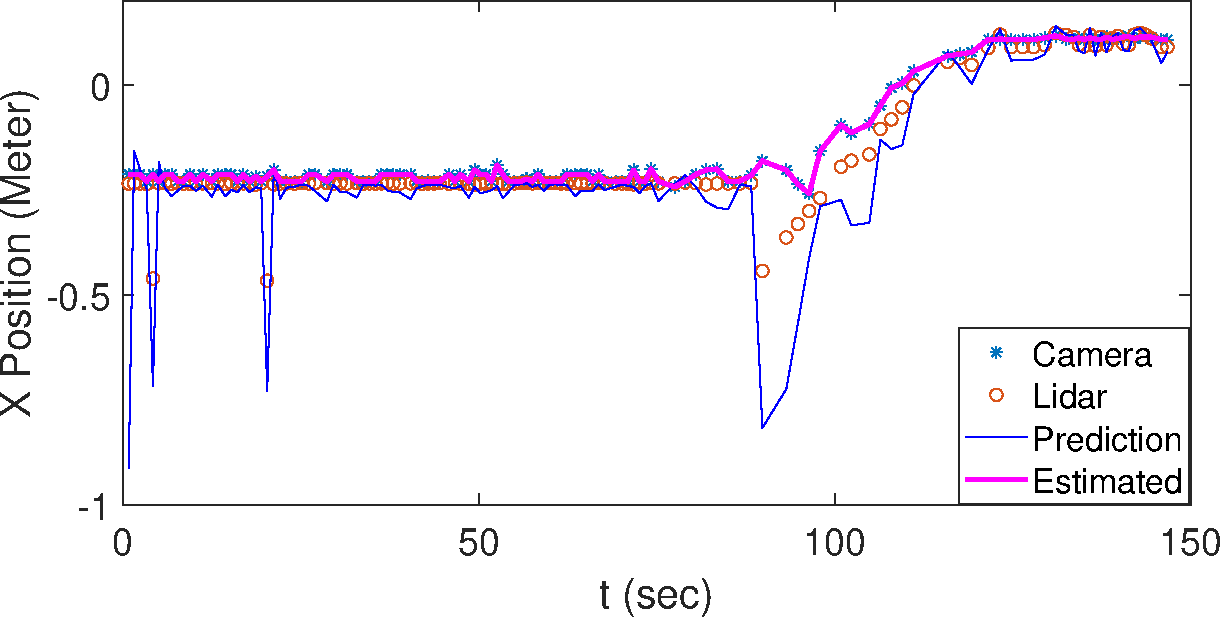
\includegraphics[height=6.5cm,width=0.9\textwidth]{Images/X_postc.pdf}
    \end{subfigure}
    \begin{subfigure}
        \centering
        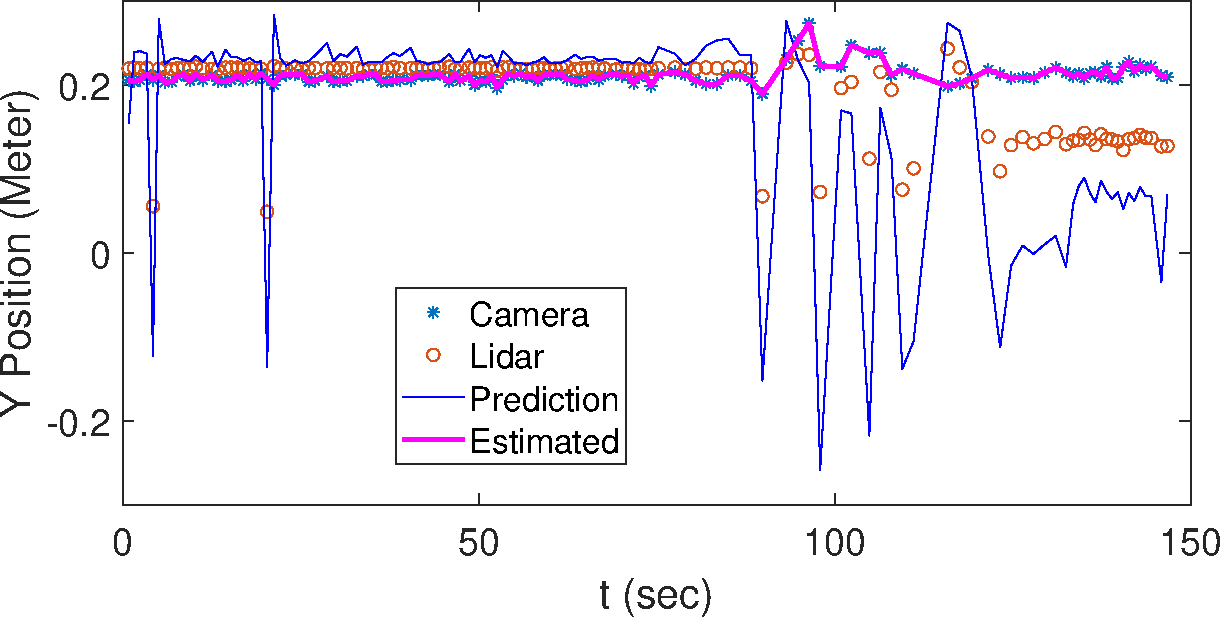
\includegraphics[height=6.5cm,width=0.9\textwidth]{Images/Y_postc.pdf}
    \end{subfigure}
    \begin{subfigure}
        \centering
        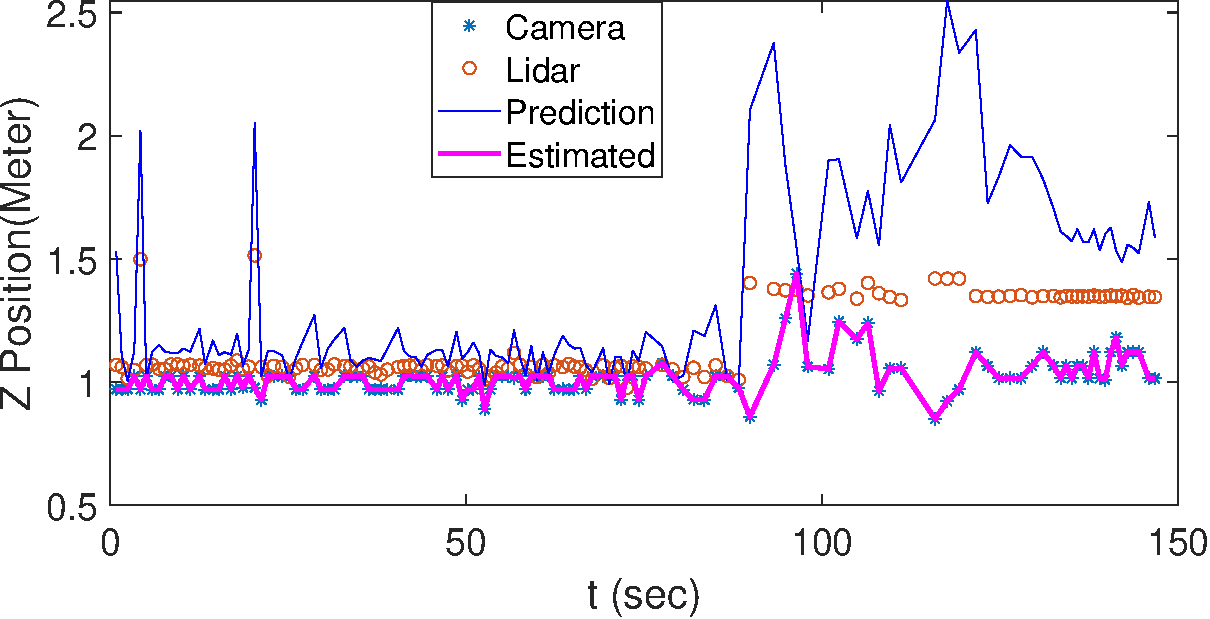
\includegraphics[height=6.5cm,width=0.9\textwidth]{Images/Z_postc.pdf}
    \end{subfigure}
    \caption{Real time Position Estimation of a Object 'Traffic cone'}
    \label{Stateesttc}
\end{figure}

\begin{figure}
    \centering
    \begin{subfigure}
        \centering
        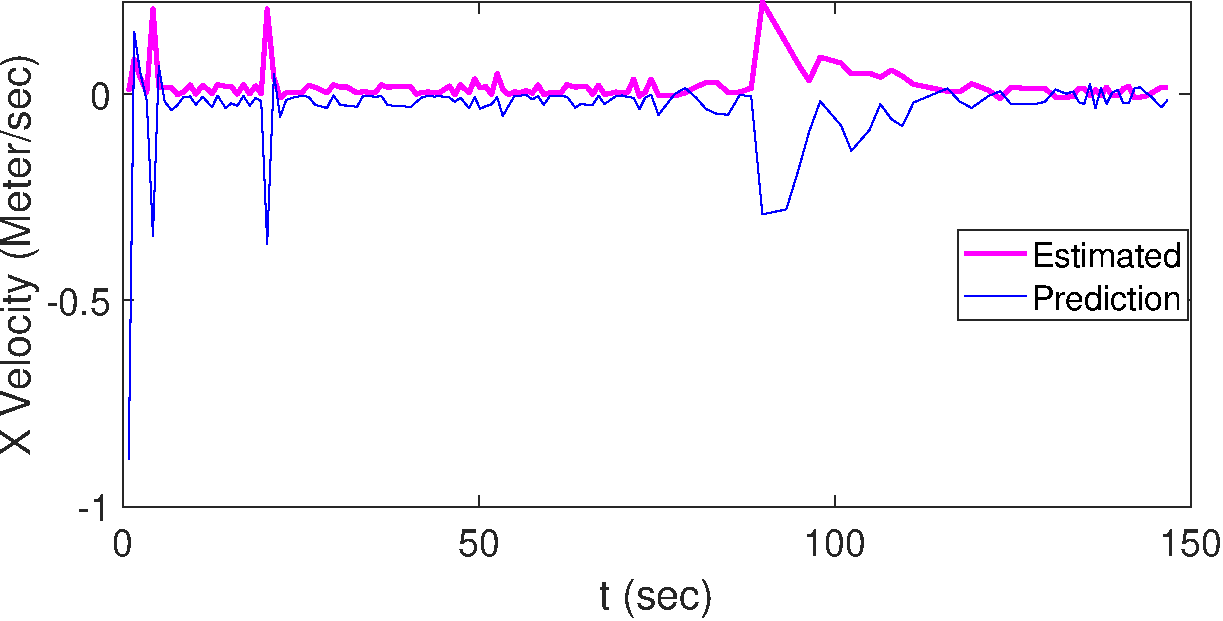
\includegraphics[height=6.5cm,width=0.9\textwidth]{Images/X_Veltc.pdf}
    \end{subfigure}
    \begin{subfigure}
        \centering
        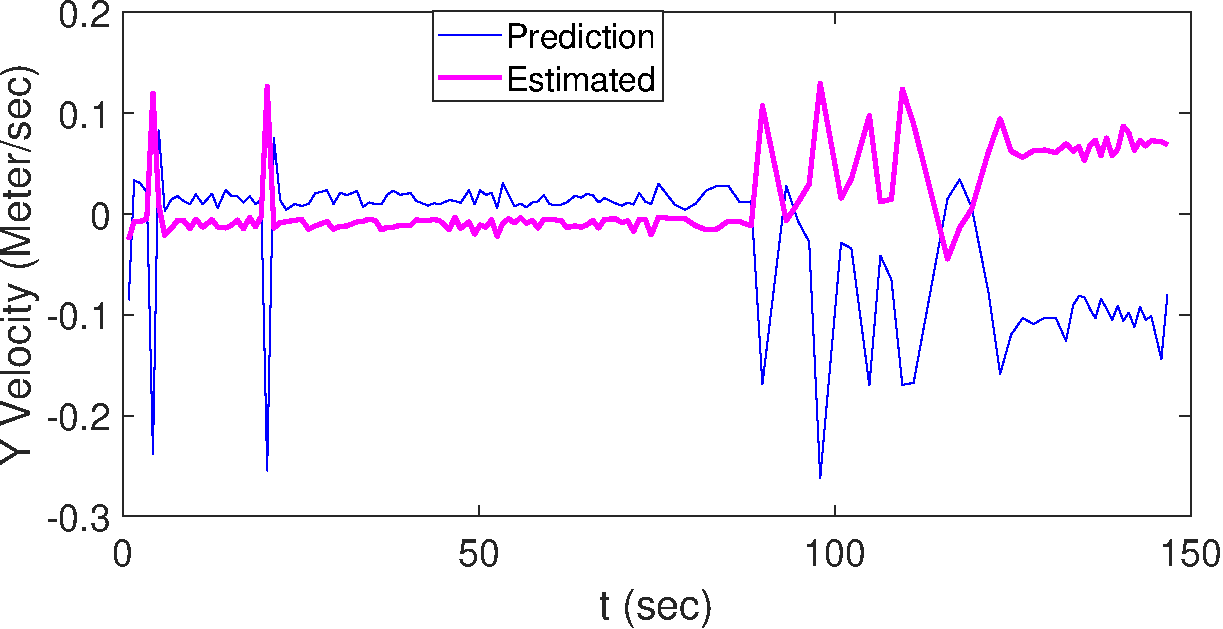
\includegraphics[height=6.5cm,width=0.9\textwidth]{Images/Y_Veltc.pdf}
    \end{subfigure}
    \begin{subfigure}
        \centering
        \includegraphics[height=6.5cm,width=0.9\textwidth]{Images/Z_Veltc.pdf}
    \end{subfigure}
    \caption{Real time Velocity Estimation of a Object 'Traffic cone'}
    \label{Veloesttc}
\end{figure}


\begin{figure}
    \centering
    \begin{subfigure}[]
        \centering
        \includegraphics[width=0.45\textwidth]{Images/Cy_d86cm.PNG}
    \end{subfigure}
    \begin{subfigure}[]
        \centering
        \includegraphics[width=0.45\textwidth]{Images/Cy_d91cm.PNG}
    \end{subfigure}
    \begin{subfigure}[]
        \centering
        \includegraphics[width=0.45\textwidth]{Images/Py_d103cm.PNG}
    \end{subfigure}
    \begin{subfigure}[]
        \centering
        \includegraphics[width=0.45\textwidth]{Images/Box_d94cm.PNG}
    \end{subfigure}
    \begin{subfigure}[]
        \centering
        \includegraphics[width=0.45\textwidth]{Images/TC_d97cm.PNG}
    \end{subfigure}
    \begin{subfigure}[]
        \centering
        \includegraphics[width=0.45\textwidth]{Images/TC_d103cm.PNG}
    \end{subfigure}    
    \caption{Real time Object Detection and Position Estimation of Various Object}
    \label{realtimeestimation}
\end{figure}



\section{Conclusion}
It was shown in this work that the YOLO-v3 unified algorithm performs better and faster than most of the modern object detection neural networks. An intrinsic and extrinsic calibration of LiDAR and stereo camera was carried out to compute the measurement and transformation error of camera and LiDAR data. This was shown to be 0.3 m for the camera to LiDAR and LiDAR to camera transformation and -0.004 m and -0.021 m for camera and LiDAR transformation.

A labeled training data-set of 11000 images was created to train YOLO-v3 deep neural network so that it can detect four basic shapes: cylinder, cone, pyramid, and box. The data-set of 11000 images was randomly divided so that \(98\%\) of the data-set can be used for training and the other \(2\%\) can be used for validation of the trained neural network. The hyper-parameters like L2 regularization, minimum batch size, number of epoch, etc. were finely tuned to train the neural network faster with precision. The labeled data-set for LiDAR was generated by using the image label and creating the bounding boxes on LiDAR data based on the known depth of the obstacles. Finally, a sensor fusion algorithm was implemented by using a linear Kalman filter to fuse the data coming from LiDAR and the stereo camera.

\newpage
\section{Future Work}
This study has covered a broad aspect of the field of computer vision, deep learning, statistics, and practical implementation. To cover greater depth in each mentioned field is difficult due to time constrains; however, this study lays down a ground for further advanced research. Some suggestions for possible future work are listed as follows. 

\begin{itemize}
    \item Develop a more sophisticated multi-object tracking algorithm; for instance JPDA (Joint Probabilistic Data Association). 
    \item Further this study can be extended to implement the collision avoidance, and SLAM (Simultaneous Localization and Mapping).
    \item The neural network can be trained to detect more complex objects that might be encountered in the real world.
    \item The YOLO-v3 network can be further tuned to improve test accuracy.
    \item By use of the LiDAR with a stronger laser that can be used in ambient conditions, this research work can be extended to autonomous driving or advanced driving assistance system.
    \item The LiDAR and camera calibrations can be automated and made more accurate to improve the overall system accuracy in the future. 
\end{itemize}
 



